%%%%%%%%%%%%%%%%%%%%%%%%%%%%%%
%
%      Apuntes de la asignatura de Control y Programación de Robots
%       Robot Control and Programming: Class notes
%      Autor: Emilio José Sánchez Tapia
%      Fecha: Junio 2008
%
%%%%%%%%%%%%%%%%%%%%%%%%%%%%%%

% el documento tiene estructura de libro
\documentclass[a4paper,twoside, 11pt]{book}

%configuraciones de idioma, márgenes y encabezados
\input{preamble}

\newcommand{\CPRindex}[1]{\textit{\textbf{#1}}\index{#1}}

\hyphenpenalty 1000

\begin{document}


%añade portada
\frontmatter
\graphicspath{{./}}
\begin{titlepage}
	%\ThisCenterWallPaper{1}{figuras/SKILLS_portada.pdf}
\begin{center}
	\vspace*{-1.35in}
	\begin{figure}[htb]
		\begin{center}
			
\includegraphics{tecnun.png}
		\end{center}
	\end{figure}

	\vspace*{0.8in}
	\large{MASTER THESIS}

	\large{\textbf{INDUSTRIAL ENGINEERING}}
       
  	\vspace{2in}
    \Huge{\textbf{ROBOTIC STRING-ENVELOPE OPENING}}
	~ \vfill
\end{center}

	\raggedleft{Irune Goizueta Zubimendi}\\
 	\raggedleft{San Sebasti\'an, April 2018}
	
 
\end{titlepage}


%\maketitle
%\thispagestyle{plain}

%preparación del índice
\setcounter{tocdepth}{2} %inserta todos los títulos hasta el nivel \subsection{} en la tabla de contenidos
\setcounter{secnumdepth}{3} %numera todos los títulos hasta el niver \subsubsection{}

\tableofcontents % tabla de contenidos
\newpage
\listoffigures %índice de figuras
\newpage
\listoftables %índice de tablas
\newpage


% insertar la lista de notación
%\printglossary
%\newpage



\chapter{ABSTRACT}
\label{ch:abstract}

Robotic manipulation of deformable objects is a challenging subject and can often be bothersome. The behavior of this kind of objects is difficult to predict because they are constantly changing their shape when they are exposed to external forces. However, deformable objects such as ropes, wires, strings, cloths, are present in industry and in our daily lifes. For that reason, we decided to focus our research on robotic manipulation of deformable objects. This project has been developed at the Robotics Institute of the Hong Kong University of Science and Technology during a period of six months. The goal of this project is to open an arbitrarily tied string-envelope with a UR10 robot, using a Robotiq FT300 wrist force/torque sensor. 



%comienzo del libro
\mainmatter


%Configuración particular de las cabeceras y pies de página del mainmatter
\renewcommand{\chaptermark}[1]{\markboth{Chapter \thechapter. #1}{}} %configuración de las cabeceras
\renewcommand{\sectionmark}[1]{\markright{Section \thesection. #1}}
\renewcommand{\headrulewidth}{0.4 pt} %modifica el ancho de las líneas de cabecera 
\renewcommand{\footrulewidth}{0 pt} % el pie sin línea


%\part{INTRODUCTION}

%%%%%%%%%%%%%%% Chapters

%introducci'on general 
\chapter{INTRODUCTION}
\label{ch:introduction}
In this chapter we introduce the work that has been done at the Robotics Institute of the Hong Kong University of Science and Technology (HKUST) during a period of six months. We focus on robotic manipulation of deformable objects. We explain here the motivation to do this work and its goal.

\section{Motivation}
Let's start by talking about robotic manipulation. The research about this topic has become increasingly popular over the last 50 years \cite{fanson2010robotic}, especially for industrial applications that focus on the execution of repetitive tasks, tasks that require big efforts, high precision or that are dangerous. This period has been accompanied by a technological maturation of robots as well, from the simple pick and place and painting and welding robots, to more sophisticated assembly robots for inserting integrated circuit chips onto printed circuit boards, to mobile carts for parts handling and delivery \cite{murray2017mathematical}. Several areas of robotic automation have now become \enquote{standard} on the factory floor, but until now, most of the research on robotic manipulation assumed the handled objects to be rigid. 

However, many important application domains require manipulating deformable objects, especially deformable linear objects (DLOs), such as ropes, cables, wires, strings and sutures. Such objects can be found almost everywhere in the real world of industry and in human daily life and they are far more challenging to handle, as they can exhibit a much greater diversity of behaviors \cite{saha2007manipulation}. They add a number of difficulties to the manipulation task by continuously changing shape when exposed to external forces. 

There have already been studies about robotic manipulation of deformable linear objects. For example, \cite{saha2007manipulation} describes a motion planner for manipulating DLOs and tying knots (self-knots and knots around simple static objects) using two cooperating robot arms. Then, \cite{yue2001manipulating} and \cite{yue2002manipulating} analyze how to adjust the motion during the manipulation of a DLO in order to eliminate vibration.

For this project, we want to continue in the same line as the works mentioned but focusing on a new problem that has not been studied before. 

\section{Project Goal}
To determine the goal of this project we started with some limitations: the material available. The material provided to work with is mentioned below:
\begin{itemize}
	\item Universal Robots UR10 robot arm.
	\item Robotiq Force Torque Sensor FT 300.
	\item Robotiq 3-Finger Adaptative Robot Gripper.
\end{itemize}

The UR10 robot arm used in this project is shown in Figure~\ref{fig:ur10} below:
\begin{figure}[h!]
	\centering
	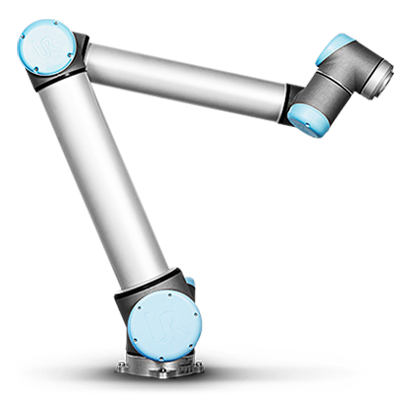
\includegraphics[height=80mm]{chapters/figures/intro/ur10.jpg}
	\caption{Universal Robots UR10 Robot Arm.}
	\label{fig:ur10}
\end{figure}\\
This is the larger industrial robot arm of the Universal Robots and it is designed for bigger tasks where precision and reliability are still of paramount importance. The UR10 robot arm allows to automate processes and tasks with payloads that weigh up to 10 kg. It has 6 degree-of-freedom and it can follow position commands like a traditional industrial robot, as well as take force commands to apply a given force or torque in/around a specified axis. In addition to standard programming, this robot has a freedrive mode for tactile programming \cite{universalrobots2014ur10}.

Attached to the wrist of the UR10 robot arm, we find the Robotiq Force Torque Sensor FT 300, shown in Figure~\ref{fig:ft300}:\\
\begin{figure}[h!]
	\centering
	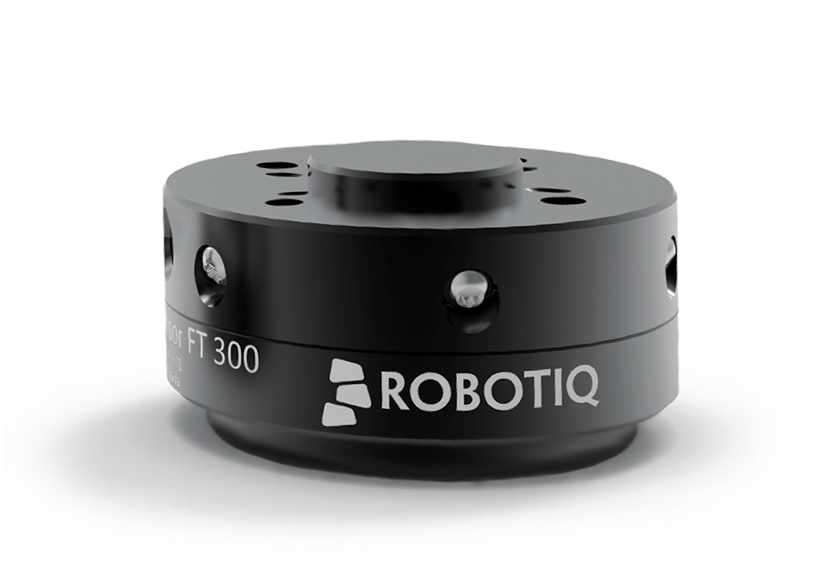
\includegraphics[height=45mm]{chapters/figures/intro/ft300.jpg}
	\caption{Robotiq Force Torque Sensor FT 300.}
	\label{fig:ft300}
\end{figure}\\
The FT sensor is meant to have an end-of-arm tool mounted on it, so that it can sense force and torque applied on the tool. The sensor is compatible with various tools and provides feedback that can be used for: hand guiding a robot, force control processes, assembly tasks, product testing, etc \cite{robotiq2016ftsensor}.

The tool mounted on the FT 300 sensor is the Robotiq 3-Finger Adaptative Robot Gripper, shown in Figure~\ref{fig:gripper}:
\begin{figure}[htbp]
	\centering
	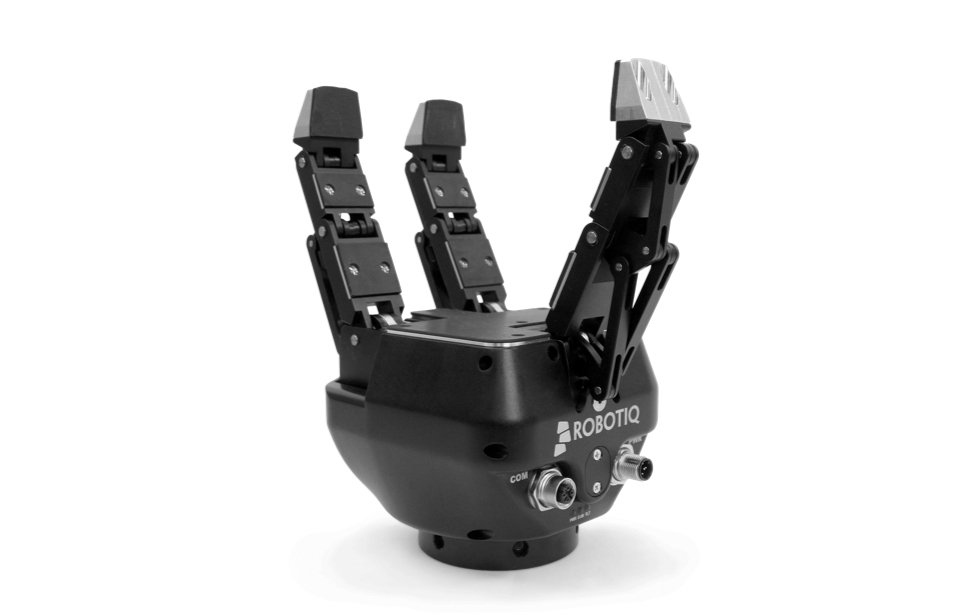
\includegraphics[height=60mm]{chapters/figures/intro/gripper.jpg}
	\caption{Robotiq 3-Finger Adaptative Robot Gripper.}
	\label{fig:gripper}
\end{figure}\\
The Robotiq 3-Finger Adaptative Robot Gripper is a robotic peripheral that is designed for industrial applications. Its design makes it a unique robotic end-of-arm tool to pick, place and handle a large range and volume of parts of varying sizes and shapes. It has three articulated fingers, that each have three joints. The gripper can angage up to ten points of contact with an object (three on each of the phalanges plus the palm). The fingers are under-actuated, meaning they have fewer motors than the total number of joints. This configuration allows the fingers to automatically adapt to the shape of the object they grip and it also simplifies the control of the gripper \cite{robotiq2014gripper}.

With these components, we have to determine the goal of the project being conscious of the limitations.

In HKUST, string-envelopes are very commonly used to send the correspondence because they can be re-used several times. We thought that a good challenge could be to try opening a tied envelope using the robot arm. For this, we have to figure out how to untie the string that has previously been tied in an arbitrarily manner. The envelope used for this project is shown in Figure~\ref{fig:envelope}:
\begin{figure}[htbp]
	\centering
	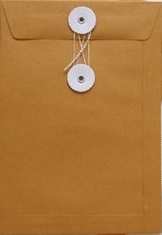
\includegraphics[height=50mm]{chapters/figures/intro/envelope.jpg}
	\caption{String-Envelope.}
	\label{fig:envelope}
\end{figure}

The initial configuration for all the components is shown in Figure~\ref{fig:assembly}:
\begin{figure}[htbp]
\centering
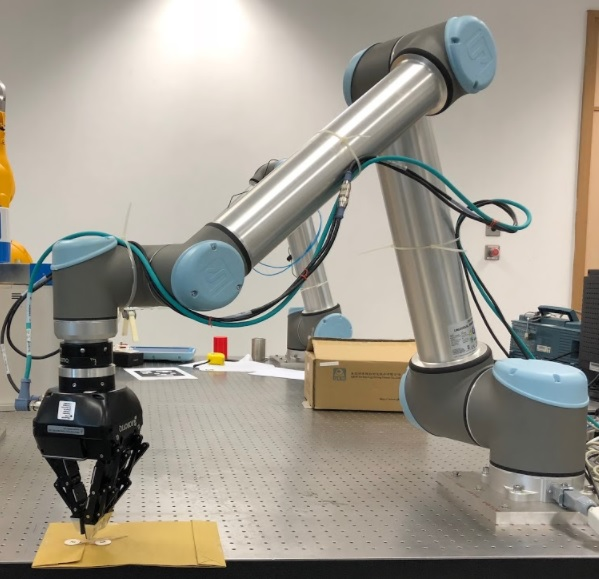
\includegraphics[height=100mm]{chapters/figures/intro/assembly.jpg}
\caption{Assembly of the elements to compose the initial configuration of the robot.}
\label{fig:assembly}
\end{figure}

To accomplish the main goal, it is important to first achieve the following sub-goals:
\begin{itemize}
\item Learn about ROS.
\item Control UR10, Robotiq 3 finger gripper and get data from Robotiq FT300 through ROS.
\item Plan the motion for the gripper to untie the string.
\item Establish the algorithm to generalize the problem so the robot can open the envelope being tied in an arbitrarily manner.
\end{itemize}

In this document, we explain how these sub-goals were accomplished in order to achieve the main goal.

\textbf{Chapter 2} talks about ROS (Robot Operating System), system used to control the robot. It also introduces MoveIt!, which provides the core functionality for manipulation in ROS.

\textbf{Chapter 3} explains how to solve the problem for untying the string from the pivots, which path the end-effector must follow.

\textbf{Chapter 4} shows and explains the algorithm we came up with to solve the general problem of untying arbitrarily tied string-envelopes. 

\textbf{Chapter 5} shows some experiments that have been done and their results.

\textbf{Chapter 6} concludes this work and talks about future lines to continue developing this project.

We will start now to talk about ROS.



%\part{ROS}

% programaci'on de robots industriales
\chapter{ROS AND MOVEIT!}
\label{ch:ROS AND MOVEIT!}
In this chapter, we make a brief introduction to ROS \cite{o2014gentle}, system we used to program the robot arm, the force/torque sensor and the gripper. We also talk about MoveIt!, which provides the functionality for manipulation in ROS.

\section{Introduction to ROS}
The rapid progress on the development of robotic systems has caused that robots still present some significant challenges for software developers. ROS, Robot Operating System, is a platform that is intended to ease some of these difficulties. The official description of ROS is:
\begin{quote}
\textit{ROS is an open-source, meta-operating system for your robot. It provides the services you would expect from an operating system, including hardware abstraction, low-level device control, implementation of commonly-used functionality, message-passing between processes, and package management. It also provides tools and libraries for obtaining, building, writing, and running code across multiple computers. \cite{o2014gentle}}
\end{quote}

Creating truly robust, general-purpose robot software is hard. From the robot's perspective, problems that seem trivial to humans often vary wildly between instances of tasks and environments. Dealing with these variations is so hard that no single individual, laboratory, or institution can hope to do it on their own \cite{ros}.

The Robot Operating System (ROS) is a flexible framework for writing robot software. It is a collection of tools, libraries, and conventions that aim to simplify the task of creating complex and robust robot behavior across a wide variety of robotic platforms \cite{cashmore2015rosplan}.

The goal of ROS is not to be a framework with the most features. Instead, the primary goal of ROS is to support code reuse in robotics research and development. ROS is a distributed framework of processes (aka Nodes) that enables executables to be individually designed and loosely coupled at runtime. These processes can be grouped into Packages and Stacks, which can be easily shared and distributed. ROS also supports a federated system of code Repositories that enable collaboration to be distributed as well. This design, from the filesystem level to the community level, enables independent decisions about development and implementation, but all can be brought together with ROS infrastructure tools \cite{wikiros}.

As a result, ROS was built from the ground up to encourage collaborative robotics software development. For example, one laboratory might have experts in mapping indoor environments, and could contribute a world-class system for producing maps. Another group might have experts at using maps to navigate, and yet another group might have discovered a computer vision approach that works well for recognizing small objects in clutter. ROS was designed specifically for groups like these to collaborate and build upon each other's work \cite{ros}.

We can thus say that the advent of new open-source frameworks like ROS has made robotics more accessible to new users, both in research and consumer applications. ROS has revolutionized the developers community, providing it with a set of tools, infrastructure and best practices to build new applications and robots. A key pillar of the ROS effort is the notion of \textit{not re-inventing the wheel} by providing easy to use libraries for different capabilities like navigation, manipulation, control (and more) \cite{koubaa2016robot}.

Figure~\ref{fig:ros} below summarizes ROS:

\begin{figure}[htbp]
	\centering
	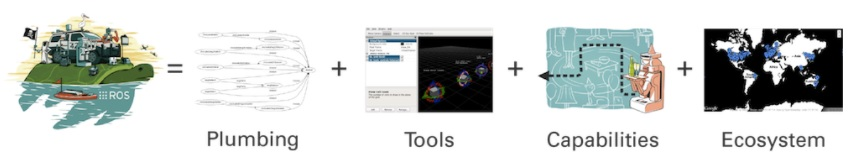
\includegraphics{chapters/figures/ROS/ROS.jpg}
	\caption{ROS Summary.}
	\label{fig:ros}
\end{figure}

\textit{Plumbing:} ROS provides publish-subscribe messaging infrastructure designed to support the quick and easy construction of distributed computing systems.

\textit{Tools:} ROS provides an extensive set of tools for configuring, starting, introspecting, debugging, visualizing, logging, testing, and stopping distributed computing systems.

\textit{Capabilities:} ROS provides a broad collection of libraries that implement useful robot functionality, with a focus on mobility, manipulation, and perception.

\textit{Ecosystem:} ROS is supported and improved by a large community, with a strong focus on integration and documentation. ros.org is a one-stop-shop for finding and learning about the thousands of ROS packages that are available from developers around the world.

 ROS has already been implemented in Python, C++, and Lisp, and there are experimental libraries in Java and Lua \cite{wikiros}.

ROS currently only runs on Unix-based platforms. Software for ROS is primarily tested on Ubuntu and Mac OS X systems, though the ROS community has been contributing support for Fedora, Gentoo, Arch Linux and other Linux platforms. While a port to Microsoft Windows for ROS is possible, it has not yet been fully explored \cite{wikiros}.

As this project focuses on robotic manipulation, let's now talk about MoveIt! which provides the core functionality for manipulation in ROS.

\section{MoveIt!}
MoveIt! is a software for mobile manipulation, incorporating the latest advances in motion planning, manipulation, 3D perception, kinematics, control and navigation. It provides an easy-to-use platform for developing advanced robotic applications, evaluating new robot designs and building integrated robotics products for industrial, commercial, R\&D and other domains \cite{moveit}. 

This software builds on multiple pillars:
\begin{itemize}
\item A library of capabilities: MoveIt! provides a library of robotic capabilities for manipulation, motion planning, control and mobile manipulation.
\item A strong community: A strong community of users and developers that help in maintaining and extending MoveIt! to new applications.
\item Tools: A set of tools that allow new users to integrate MoveIt! with their robots and advanced users to deploy new applications.
\end{itemize}

MoveIt! is the most widely used open-source software for manipulation and has been used on over 65 different robots \cite{koubaa2016robot}. 

\begin{figure}[htbp]
	\centering
	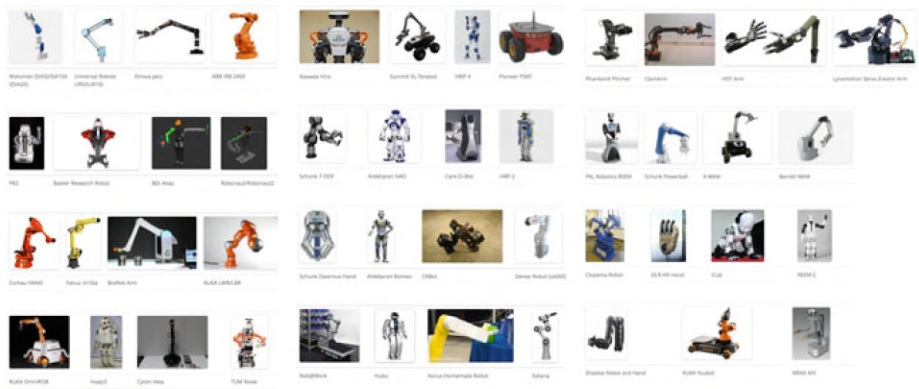
\includegraphics{chapters/figures/ROS/robots_moveit.jpg}
	\caption{Robots using MoveIt!}
	\label{fig:robots_moveit}
\end{figure}

Figure~\ref{fig:robots_moveit} shows a list of robots that MoveIt! has been used with. The robots range from industrial robots from all the leading vendors to research robots from all over the world. The robots include single arm, dual-armed robots, mobile manipulation systems, and humanoide robots. Among these robots, we find the UR10 robot arm which we will be working with. MoveIt! has been used in applications ranging from unstructured autonomous pick and place (with industrial robots like the UR5), mobile manipulation (with the PR2 and other robots), process tasks like painting and welding, with the (simulated) Robonaut robot for target applications in the space station. MoveIt! has been used used by teams in the DARPA Robotics Challenge, the ROS-Industrial Consortium, the Amazon Picking Challenge, the NASA sample retrieval challenge \cite{koubaa2016robot}.

\section{How to control to UR10, Robotiq 3 finger gripper and Robotiq FT300 force/torque sensor through ROS}
In this section, we explain how to control UR10, Robotiq 3 finger gripper and FT300 force/torque sensor through ROS.
%
%For this project, we are working on Ubuntu 16.04.3 LTS with ROS kinetic.

To control UR10 through ROS, we must install the Universal Robots package \cite{urpackage}. Through this package we can establish communication with UR10 controllers. Then, for the communication with Robotiq FT300 force/torque sensor and the 3 finger gripper, we must install Robotiq package \cite{robotiq}. Once we have installed those packages, we can run the executables to establish the connection with the three elements.

To make the connection with UR10 robot, the files shown below must be launched in three different terminals:
\begin{quote}
\textit{roslaunch ur\_modern\_driver ur10\_bringup.launch limited:=true robot\_ip:=192.168.1.102 [reverse\_port:=REVERSE\_PORT]}

\textit{roslaunch ur10\_moveit\_config ur10\_moveit\_planning\_execution.launch limited:=true}

\textit{roslaunch ur10\_moveit\_config moveit\_rviz.launch config:=true}
\end{quote}

Now we can create an executable to move the robot arm through ROS.

The communication with the FT300 is made by typing in two different terminals:
\begin{quote}
\textit{sudo chmod 777 /dev/ttyUSB1}

\textit{rosrun robotiq\_force\_torque\_sensor rq\_sensor}
\end{quote}

And the connection with the gripper is made by typing in other two different terminals:
\begin{quote}
\textit{rosrun robotiq\_s\_model\_control SModelTcpNode.py 192.168.1.11}

\textit{rosrun robotiq\_s\_model\_control SModelSimpleController.py}
\end{quote}

Now, we know how to control the three elements through ROS, so let's figure out which path the end-effector must follow to untie the string.


%\part{MOTION PLANNING}
% programaci'on de robots industriales
\chapter{MOTION PLANNING}
\label{ch:Motion planning}
In this chapter we explain the solution to plan the trajectory of the end effector in order to unwound the string from the pivots.

\section{Involute of a circle}
Let's start talking about the involute of a circle. This one was discovered in 1673 by Christiaan Huygens, a Dutch mathematician and physicist. In his work titled "Horologium oscillatorium sive de motu pendulorum ad horologia aptato demonstrationes geometricae", he focused upon the theories about the motion of pendulum. He was interested in making clocks for ships at sea. Finding a clock which would keep accurate time at sea was a major problem and many years were spent looking for a solution. This issue was of vital importance since if GMT was known from a clock then, since local time could be easily computed from the sun, longitude could be easily computed.  He introduced there the concept of involute or evolvent of the curve and he used the circle involute in his first pendulum clock in an attempt to force the pendulum to swing in the path of a cycloid \cite{mccleary2013geometry}. 

%The problem was that it was not possible to have a normal oscillating pendulum in these clocks as the rocking of ships on sea would alter the pendulum movements. Therefore there had to be a way for clocks without pendulums to show correct time. He introduced there the concept of involute or evolvent of the curve and he used the circle involute in his first pendulum clock in an attempt to force the pendulum to swing in the path of a cycloid. 

In differential geometry, the involute is defined as a curve that is obtained by attaching an imaginary string and winding or unwinding it tautly on the given curve. The locus of the free end of this attached taut string is known as an involute or an evolvent  \cite{mccleary2013geometry}.

The involute of a given curve can also be defined as a line segment that is tangent to the curve on one end, while the other end traces out the involute. This line segment is wound or reversely unwound along with the continuous variation in the length of line segment by a certain amount. The curve so traced by free end is called an involute  \cite{mccleary2013geometry}.

In the case of this project, we have to unwound the string from circular pivots, the solution is thus the involute of a circle. This is the curve traced by the free end of a thread unwound from a circle in such a way that the thread is always tight and tangential to the circle. More practically, it is the curve traced by a hand unwinding a wire reel held in the other hand.

In this curve, all the normals are tangent to a fixed circle. Conversely, if an involute of a circle turns around the centre of the generating circle, every tangent to the circle remains always normal to the involute.

Figure~\ref{fig:involute} below shows how the involute of a circle looks like:

\begin{figure}[htbp]
	\centering
	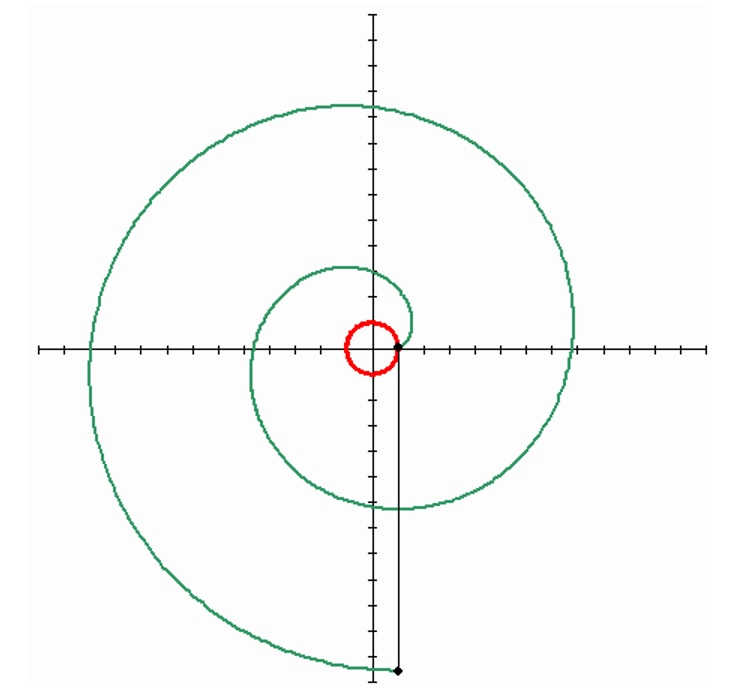
\includegraphics[height=70mm]{chapters/figures/motion_planning/involute.jpg}
	\caption{Involute of a circle.}
	\label{fig:involute}
\end{figure}

Its parametric equations in the Cartesian coordinates are:
\begin{equation*}
\begin{split}
x = a \cdot (cos(t) + t \cdot sin(t)) \\ 
y = a \cdot (sin(t) - t \cdot cos(t))
\end{split}
\end{equation*}

Where \textit{a} is the radius of the circle and \textit{t} is the angle in radians.

We noticed that the involute of a circle has a very similar shape to the Archimedean spiral.

\section{Archimedean spiral}
The Archimedean spiral is the asymptotic curve to the involute of a circle for large values of the angle \textit{t}. It also is its pedal with respect to the center \cite{weisstein2003pedal}.

The pedal curve results from the orthogonal projection of a fixed point on the tangent lines of a given curve. The pedal of a curve with respect to a point O (or with pole O) is the locus of the feet of the lines passing by O perpendicular to the tangents to the curve \cite{weisstein2003pedal}. 

The Archimedean spiral, also known as arithmetic spiral,  is a spiral named after the 3rd century BC Greek mathematician Archimedes. It is the trajectory of a point moving uniformly (with a constant speed) on a straight line of a plane, this line turning itself uniformly (rotating with constant angular velocity) around one of its points \cite{sloane}. It has the property that any ray from the origin intersects successive turnings of the spiral in points with a constant separation distance, hence the name "arithmetic spiral" \cite{holland1957archimedes}.

The Archimedean spiral has two arms, one for angle $t > 0\textdegree$ and one for $t < 0\textdegree$. The two arms are smoothly connected at the origin. Only one arm is shown in Figure~\ref{fig:spiral}. Taking the mirror image of this arm across the y-axis will yield the other arm.

\begin{figure}[htbp]
	\centering
	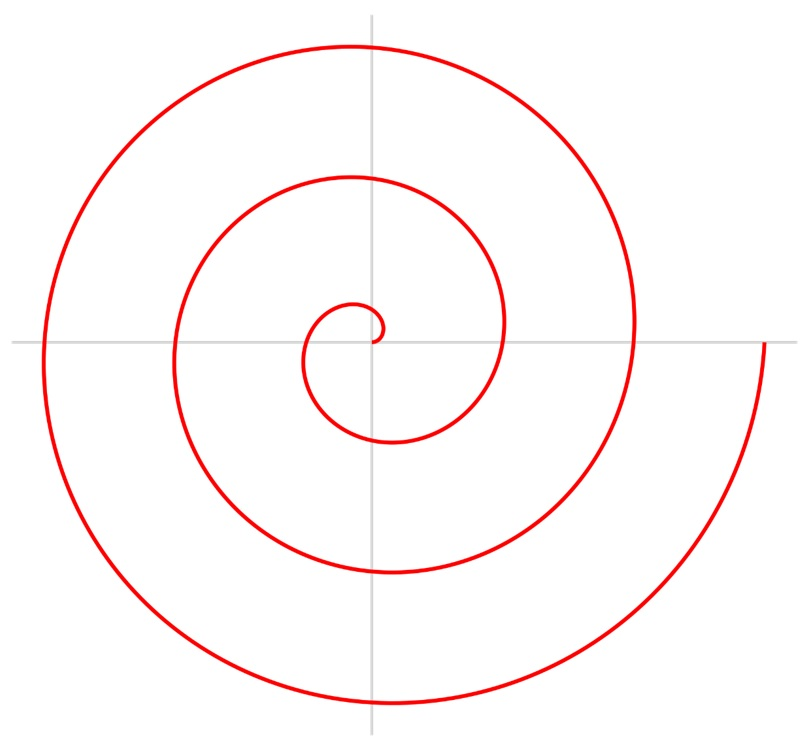
\includegraphics[height=70mm]{chapters/figures/motion_planning/spiral.jpg}
	\caption{Archimedean spiral.}
	\label{fig:spiral}
\end{figure}

Its parametric equation is the one shown below:
\begin{equation*}
\begin{split}
x = r \cdot t \cdot cos(t) \\ 
y = r \cdot t \cdot sin(t)
\end{split}
\end{equation*}

Where \textit{r} is the radius of the spiral and \textit{t} is the angle in radians.

Let's now compare the differences between the involute of a circle and the Archimedean spiral.

\section{Comparison between involute of a circle and Archimedean spiral}
As told before, involute of a circle and Archimedean spiral have very similar shapes. In this section we compare them and talk about the differences. Figure~\ref{fig:comparison} below shows the difference in both shapes.\newpage
\begin{figure}[h!]
	\centering
	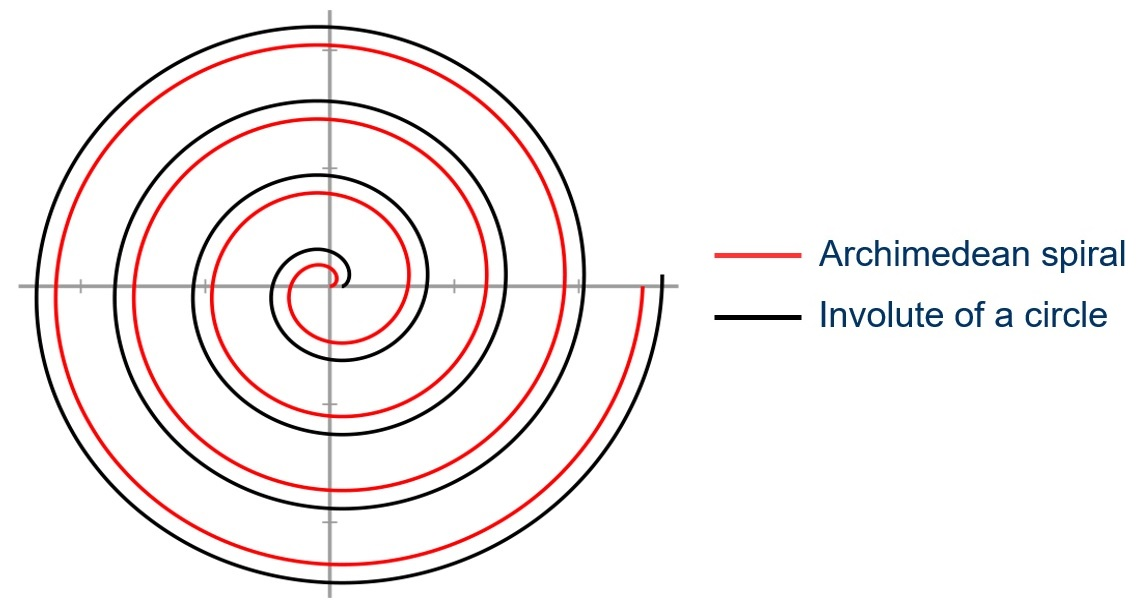
\includegraphics[height=80mm]{chapters/figures/motion_planning/comparison.jpg}
	\caption{Comparison between involute of a circle and Archimedean spiral.}
	\label{fig:comparison}
\end{figure}

Archimedean spiral is represented in red and involute of a cirlce in black. Both radius are the same, 1 unit. They seem to have the same progress as the angle increases but let's see the real differences in Table~\ref{table:comparison} below.

\begin{table}[!ht]
\begin{center}
\begin{tabular}{l|*{2}{c}r}
	                  & Archimedean spiral & Involute of a circle \\
	\hline
	Angles            & $0 \leq t \leq 8\pi$ & $0 \leq t \leq \frac{17\pi}{2}$ \\
	\hline
	Initial position  & x = 0 & x = 1 \\
	                  & y = 0 & y = 0 \\
	\hline
	Final position    & x = 25.12 & x = 26.7 \\
	                  & y = 0     & y = 1    \\
	\hline
	Equation          & $x = r \cdot t \cdot cos(t)$ & $x = a \cdot (cos(t) + t \cdot sin(t))$ \\
	                  & $y = r \cdot t \cdot sin(t)$ & $y = a \cdot (sin(t) - t \cdot cos(t))$ \\
\end{tabular}
\end{center}
\caption{Comparison between involute of a circle and Archimedean spiral.}
\label{table:comparison}
\end{table}

Let's comment the values on the table. 

If we look at Figure~\ref{fig:comparison}, both curves seem to finish almost at the same angle. However, if we look to the values on the table, we see that involute of a circle finishes $\frac{\pi}{2}$ later than the Archimidean spiral.

Concerning initial and final positions, we appreciate that the difference at the beginning is 1 unit, but at the end the difference is almost 1.6 units. We can say thus that in 4 turns, the difference between involute of a circle and Archimedean spiral increases around 0.6 units, this is 0.6/4 = 0.15 units in each turn.

Finally, if we compare both equations, we see that the equation for Armchimidean spiral is much more easy to understand and to apply than the one for involute of a circle.

As the radius of our pivots is small (0.4 mm) and the length of the string (34 cm) and distance between pivots (4.25 cm) limit the number of turns (to 5 or 6 maximum), Archimidean spiral and involute will have very similar results. So, as the equation for Archimidean spiral is easier to apply, we decide to use this one in this project in order to untie the string from the circular pivots.

Let's now show and explain the algorithm we came up with to open the string-envelope.

%\include{1_robot_intro/CPR_introduction}
%%%%%%%%%%%%%%%%%%%%%%%%%%%%%%%%%\include{3_haptics_teleoperacion/4_arquitecturas_de_teleoperacion}

%%%%%%%%%%%%%%%%% Exercises
%\part{THE ALGORITHM}

\chapter{THE ALGORITHM}
\label{ch:Algorithm}
In this chapter we explain the algorithm we came up with to open a string-envelope. The analysis of this algorithm is based on \cite{cormen2009introduction}. We start by showing the initial configuration of the robot, then we explain the algorithm by showing the flowchart followed by the pseudocode and we finish by showing some examples. The output is that the robot opens the envelope that has been previously tied in an arbitrary manner. 

\section{Initial configuration}
In this section, we show the initial configuration of all the elements and the preconditions we need for the algorithm to work correctly.

The initial configuration is shown in Figure~\ref{fig:configuration} below.
\begin{figure}[h!]
	\centering
	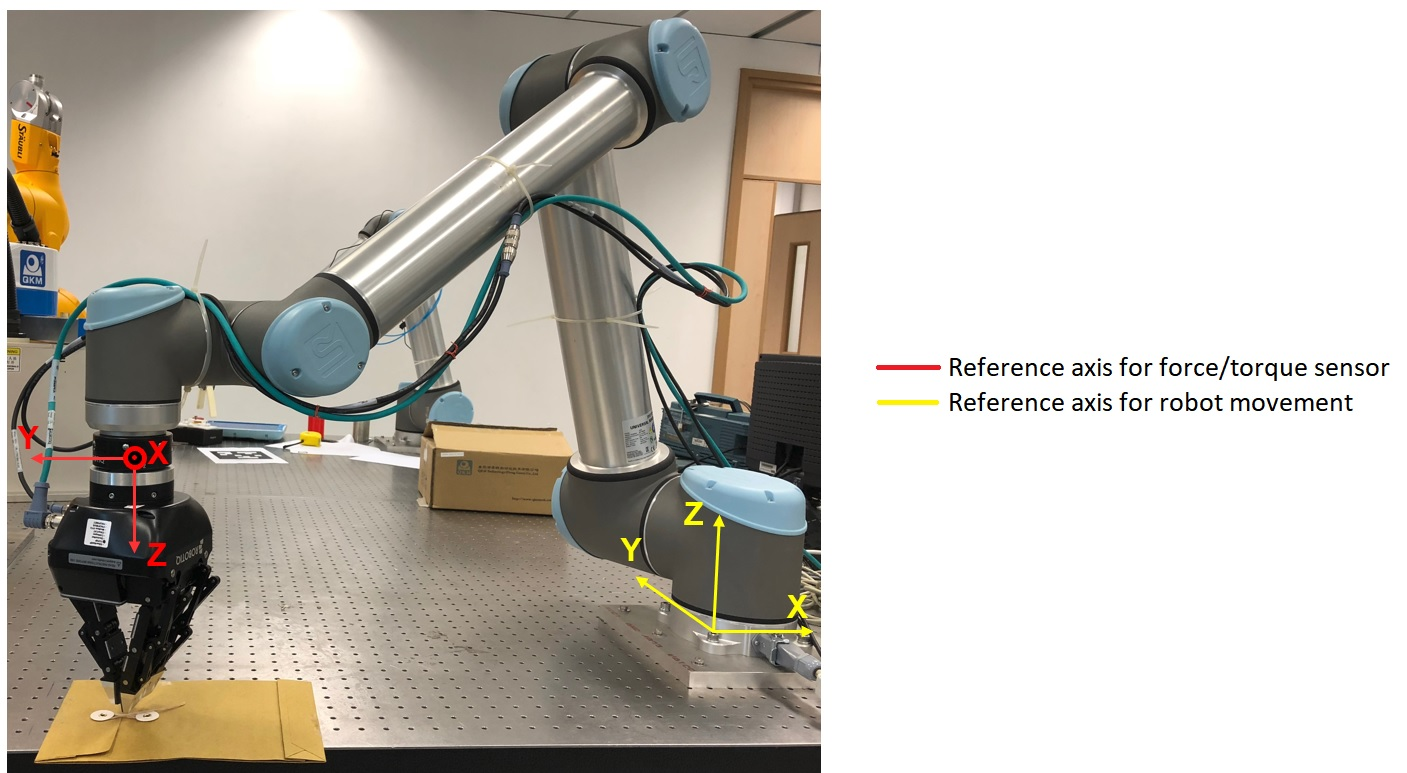
\includegraphics[height=86mm]{chapters/figures/algorithm/configuration.jpg}
	\caption{Initial configuration of the robot and all the elments.}
	\label{fig:configuration}
\end{figure}

The red axis represents the reference for the wrist force-torque sensor and the yellow axis represents the reference for the robot movement.

The preconditions for the algorithm to work are:
\begin{itemize}
 \item The robot is already grasping the string in the middle between the two pivots.
 \item $r_{p}$: Pivots' radius.
 \item $d$: Distance between pivots.
 \item $k$: Threshold value from which the torque sensor reading is considered relevant.
\end{itemize}

We call Pivot 1 to the pivot that is attached to the flap of the envelope and Pivot 2 to the other one. We will use the abbreviation P1 for Pivot 1 and P2 for Pivot 2.

\section{Algorithm}
In this section, we show the flowchart, the pseudocode of the algorithm and some examples to explain how this one works.

\subsection{Flowchart}
The flowchart is shown in Figure~\ref{fig:flowchart}.

% Define block styles
\tikzstyle{decision} = [diamond, aspect=3, draw, fill=blue!20, 
text width=10em, text badly centered, node distance=3cm, inner sep=0pt]
\tikzstyle{block} = [rectangle, draw, fill=blue!20, 
text width=12em, text centered, rounded corners, minimum height=2em]
\tikzstyle{line} = [draw, -latex']
%\tikzstyle{cloud} = [draw, ellipse,fill=red!20, node distance=3cm, minimum height=2em]
\begin{figure}[h]
\begin{center}
\begin{tikzpicture}[node distance = 2.5cm, auto]
% Place nodes
\node [block] (init) {Start};
\node [block, below of=init, node distance=1.8cm] (move) {Move $2 \cdot r_{p}$ in perpendicular to pivots' joining axis};
\node [block, left of=move, node distance=5.5cm] (return) {Return to initial pose};
\node [decision, below of=move, node distance=2.2cm] (evaluate) {$|M_{x}| \geq |k|$ and $|M_{y}| \geq |k|$?};
\node [block, below of=evaluate, node distance=2.6cm] (decide) {Turn 360$\,^{\circ}$ about the right pivot in the right direction};
\node [decision, below of=decide, node distance=2.2cm] (evaluate1) {$|M_{y}| \geq |k|$?};
\node [block, below of=evaluate1,  node distance=2.4cm] (move1) {Move $2 \cdot r_{p}$ in perpendicular and outwards pivots joining axis};
\node [block, left of=move1, node distance=5.5cm] (same_pivot) {Turn 360$\,^{\circ}$ about the same pivot in the same direction};
\node [decision, below of=move1, node distance=2.4cm] (evaluate2) {$|M_{y}| \geq |k|$?};
\node [block, below of=evaluate2,  node distance=2.5cm] (opsd) {Turn in the same direction about the opposite pivot};
\node [block, left of=opsd, node distance=5.5cm] (opod) {Turn in the opposite direction about the opposite pivot};
\node [decision, below of=opsd, node distance=2.5cm] (evaluate3) {Gripper turning about P1?};
\node [block, right of=evaluate3, text width=9em, node distance=6cm] (continue) {Keep going until turn complete};
\node [decision, below of=evaluate3, node distance=2.8cm] (evaluate4) {$|M_{x}| \geq |k|$ or $|M_{y}| \geq |k|$?};
\node [block, left of=evaluate4, text width=6em, node distance=6cm] (stop) {Stop};

% Draw edges
\path [line] (init) -- (move);
\path [line] (move) -- (evaluate);
\path [line] (evaluate) -| node [near start] {no} (return);
\path [line] (return) |- (move);
\path [line] (evaluate) -- node {yes}(decide);
\path [line] (decide) -- (evaluate1);
\path [line] (evaluate1) -| node [near start] {yes} (same_pivot);
\path [line] (same_pivot) |- (evaluate1);
\path [line] (evaluate1) -- node {no} (move1);
\path [line] (move1) -- (evaluate2);
\path [line] (evaluate2) -| node [near start] {yes} (opod);
%\path [line] (opod) |- (evaluate2);
\path [line] (evaluate2) -- node {no} (opsd);
\path [line] (opod) |- (evaluate3);
\path [line] (opsd) -- (evaluate3);
\path [line] (evaluate3) -- node {no} (continue);
\path [line] (continue) |- (evaluate1);
\path [line] (evaluate3) -- node {yes} (evaluate4);
\path [line] (evaluate4) -| node [near start] {no} (continue);
\path [line] (evaluate4) -- node {yes} (stop);
\end{tikzpicture}
\end{center}
\caption{Flowchart of the algorithm to open a string-envelope.}
\label{fig:flowchart}
\end{figure}
\clearpage

The algorithm starts and the gripper moves $2 \cdot r_{p}$ in perpendicular to pivots' joining axis. If absolute values of torques around x-axis and y-axis are less than absolute value of threshold, the the gripper returns to the initial pose and it moves $2 \cdot r_{p}$ in perpendicular to pivots' joining axis, but in the opposite direction. Otherwise,  if absolute values of torques around x-axis and y-axis are greater than absolute value of threshold, then the gripper turns 360$\,^{\circ}$ about the right pivot in the right direction to untie the string, depending on the sign of torques. 

After one turn, if absolute value of torque around y-axis is greater than absolute value of threshold, then the string is tied about the same pivot and the gripper will turn 360$\,^{\circ}$ about the same pivot in the same direction. Otherwise, the gripper will move $2 \cdot r_{p}$ in perpendicular and outwards pivots' joining axis. There, if absolute value of torque around y-axis is greater than absolute value of threshold, the gripper will turn in the opposite direction about the opposite pivot to untie the string. Otherwise, the gripper will turn in the same direction about the opposite pivot to untie the string.

To know whether the string has completely been untied, it is important to know that the beginning of the string is always attached to P1. So, if the gripper is turning about P1 to try to untie the string and absolute values of torques around x-axis and y-axis increase over absolute value of threshold, then the string is completely untied and the movement stops and the algorithm ends. The fact that torque values increase during the movement about P1 means that the string has completely been untied because its length won't increase anymore while the gripper is "openning" the movement to try to untie the string.

\subsection{Pseudocode}
The pseudocode is presented as a procedure called \textbf{UNTIE-STRING} and it is shown below.
\begin{algorithm}
	\caption{UNTIE-STRING}\label{euclid}
	\begin{algorithmic}[1]
%		\Procedure{MyProcedure}{}
		\State $\textit{turn} \gets \text{0}$
		\State $[\textit{p}, \textit{c}] \gets \textbf{evaluateTorques}$
		\State Turn about \textit{p} in direction \textit{c}
		\While {True}
		\State $[\textit{p}, \textit{c}] \gets \textbf{evaluateTorques}$
		\State Turn about \textit{p} in direction \textit{c}
		\If {$\textit{p} = \textit{P1}$}
		\State Store $M_{x}$, $M_{y}$ during the movement
		\If {$|M_{x}| > \textit{k}$ or $|M_{y}| > \textit{k}$}
		\State \textbf{break}
		\Else 
		\State keep going
		\EndIf
		\EndIf
		\EndWhile
	\end{algorithmic}
\end{algorithm}

The algorithm can be divided in two parts. First part goes from line 1 to 3 and second part goes from line 4 to 12. 

The first part of the algorithm makes the first turn to start untying the string. There are four possible movements:
\begin{itemize}
	\item Rotate clockwise (CW) about P1.
	\item Rotate counterclockwise (CCW) about P1.
	\item Rotate clockwise about P2.
	\item Rotate counterclockwise about P2.
\end{itemize}

Then, for the second part of the algorithm (\textbf{while} loop), after the first turn, there are only three possible movements:
\begin{itemize}
	\item Rotate about the same pivot in the same direction.
	\item Rotate about the other pivot in the other direction.
	\item Rotate about the other pivot in the same direction.
\end{itemize}

Let's start by explaining how the algorithm makes the first movement (lines 1-3).
In line 1, the variable \textit{turn} is initialized to 0. This variable lets know whether we are in the first turn or after.
In line 2, the function \textbf{evaluateTorques} determines which pivot, \textit{p}, and direction, \textit{c}, to turn in order to untie the string, depending on torque values $M_{x}$ and $M_{y}$. This function is shown and explained later. In line 3, the first turn is executed.

After the first turn, we enter the \textbf{while} loop (lines 4-12). Here, the algorithm makes the rest of the turns and stops when the string has completely been untied. In line 5, again the \textbf{evaluateTorques} function determines the pivot \textit{p} and the direction \textit{c} to untie the string and the movement is executed in line 6. 

For the algorithm to be correct and complete, it has to determine whether the string has completely been untied or not. Once the envelope is opened, the algorithm must finish. 

As explained before, if the gripper is turning about P1 (line 7), then torques $M_{x}$ and $M_{y}$ will be stored during the movement (line 8). If torque values increase, then the movement will stop and the algorithm will finish (lines, 9, 10). 

The pseudocode for the \textbf{evaluateTorques} function is shown below:
\begin{algorithm}
	\caption{evaluateTorques}\label{euclid}
	\begin{algorithmic}[1]
		%		\Procedure{MyProcedure}{}
		\If {$\textit{turn} = 0$}
		\State $[M_{x}, M_{y}] = \textbf{pullString(0, $\pm2 \cdot r_{p}$)}$
		\If {$M_{y} > \textit{k}$ and $M_{x} < \textit{-k}$}
		\State $\textit{p} = \textit{P1}, \textit{c} = \textit{CW}$
		\ElsIf {$M_{y} > \textit{k}$ and $M_{x} > \textit{k}$}
		\State $\textit{p} = \textit{P2}, \textit{c} = \textit{CCW}$
		\ElsIf {$M_{y} < \textit{-k}$ and $M_{x} < \textit{-k}$}
	
		\algstore{myalg}
	\end{algorithmic}
\end{algorithm}

\clearpage
		
\begin{algorithm}
%	\ContinuedFloat
	\caption{evaluateTorques (continued)}
	\begin{algorithmic}
		\algrestore{myalg}
		\State $\textit{p} = \textit{P1}, \textit{c} = \textit{CCW}$	
		\ElsIf {$M_{y} < \textit{-k}$ and $M_{x} > \textit{k}$}
		\State $\textit{p} = \textit{P2}, \textit{c} = \textit{CW}$
		\EndIf
		\State $turn \hspace{0.2cm}+=1$
		\EndIf
		\If {$\textit{turn} > 0$}
		\State Store $M_{x}$, $M_{y}$
		\If {$|M_{y}| > \textit{k}$}
		\State \textit{p} and \textit{c} remain the same as in previous turn
		\Else
		\State $[M_{x}, M_{y}] = \textbf{pullString(0, $\pm2 \cdot r_{p}$)}$
		\If {$|M_{y}| > \textit{k}$}
		\State \textit{p} and \textit{c} are the opposite as in previous turn
		\Else
		\State \textit{p} is the opposite as in previous turn, \textit{c} remains the same
		\EndIf
		\EndIf
		\EndIf
		\Return {p, c}
	\end{algorithmic}
\end{algorithm}

The decision of which pivot and wich direction to turn is made inside the \textbf{evaluateTorques} function. The decision for the first turn is made from line 1 to line 11 and the decision for the rest of the turns is made from line 12 to line 21. 

For the first turn (lines 1-11), the gripper starts moving $2 \cdot r_{p}$ in perpendicular to pivots' joining axis (line 2).

Being on the right side of the pivots:
\begin{itemize}
	\item If $M_{y}$ is greater than $k$ and $M_{x}$ is less than $-k$, then the right movement to untie the string is to turn CW about P1 (lines 3, 4).
	\item If $M_{y}$ and $M_{x}$ are greater than $k$, then the right movement to untie the string is to turn CCW about P2 (lines 5, 6).
\end{itemize}

Being on the left side of the pivots:
\begin{itemize}
	\item If $M_{y}$ and  $M_{x}$ are less than $-k$, then the right movement to untie the string is to turn CCW about P1 (lines 7, 8).
	\item If $M_{y}$ is less than $-k$ and $M_{x}$ is greater than $k$, then the right movement to untie the string is to turn CW about P2 (lines 9, 10).
\end{itemize}

Then, the variable $turn$ is updated (line 11), so we know the first turn has already been made.

To figure out the rest of the turns (lines 12-21), we start by storing $M_{x}$ and $M_{y}$ values at the end of one turn (line 13). Then:

\begin{itemize}
	\item If $|M_{y}|$ is greater than $|k|$, then the gripper has to continue turning in the same direction about the same pivot to untie the string (lines 14, 15).
\end{itemize}

Otherwise, if at the end of one turn, absolute value of torque around y-axis is less than absolute value of threshold, then the string is tied about the other pivot. To know which direction to turn, the gripper will move $2 \cdot r_{p}$ in perpendicular and outwards pivots' joining axis (line 17). Then:
\begin{itemize}
	\item If $|M_{y}|$ is greater than $|k|$, then the right movement to untie the string is the opposite pivot and the opposite direction than in the previous turn (lines 18, 19).
	\item If $|M_{y}|$ is less than $|k|$, then the right movement to untie the string is the opposite pivot and the same direction than in the previous turn (lines 20, 21).
\end{itemize}

This function returns the pivot, \textit{p}, and the direction, {c}, to the main function.

After the first turn, we ignore torque around x-axis value because as the gripper unties the string and goes farther from pivots, the distance between the gripper and the pivots is much greater than the distance between pivots. As at the end of one turn the string is almost perpendicular to pivots' joining axis, torque around x-axis is almost 0 and does not allow to distinguish wich pivot to turn.

The pseudocode for the \textbf{pullString(0, $2 \cdot r_{p}$)} function (lines 2, 17), that consists of moving the gripper $2 \cdot r_{p}$ and storing $M_{x}$ and $M_{y}$, is shown below:
\begin{algorithm}
	\caption{pullString(0, $\pm2 \cdot r_{p}$)}\label{euclid}
	\begin{algorithmic}[1]
		%		\Procedure{MyProcedure}{}
		\If {$turn = 0$}
		\State Move 0 in x, $+2 \cdot r_{p}$ in y
		\If {$|M_{y}| < |k|$}
		\State Return to initial pose
		\State Move 0 in x, $-2 \cdot r_{p}$ in y
		\EndIf
		\Else
		\State Move 0 in x, $2 \cdot r_{p}$ in y outwards pivots' joing axis
		\EndIf
		\Return {$M_{x}, M_{y}$}
	\end{algorithmic}
\end{algorithm}

For the first turn (line 1), the gripper starts moving $+2 \cdot r_{p}$ in y-axis (line 2). If absolute value of torque around y-axis is less than absolute value of threshold, then the gripper returns to the initial pose and moves $-2 \cdot r_{p}$ in y-axis (lines 3-5).

After the first turn (line 6), the gripper moves $2 \cdot r_{p}$ in y-axis outwards pivots' joining axis (line 7). 

This function returns $M_{x}$ and $M_{y}$ values to the \textbf{evaluateTorques} function.

Now, we will show some examples of how the algorithm works.

\subsection{Examples}
For a better understanding of what we explained before, we show here some examples of how the algorithm works to figure out the first turn, the rest of the turns and the end of the movement. 

We start by showing an example of how the algorithm figures out the first turn. Figure~\ref{fig:first_turn} shows the four possible cases for the first turn.
\begin{figure}[h!]
	\centering
	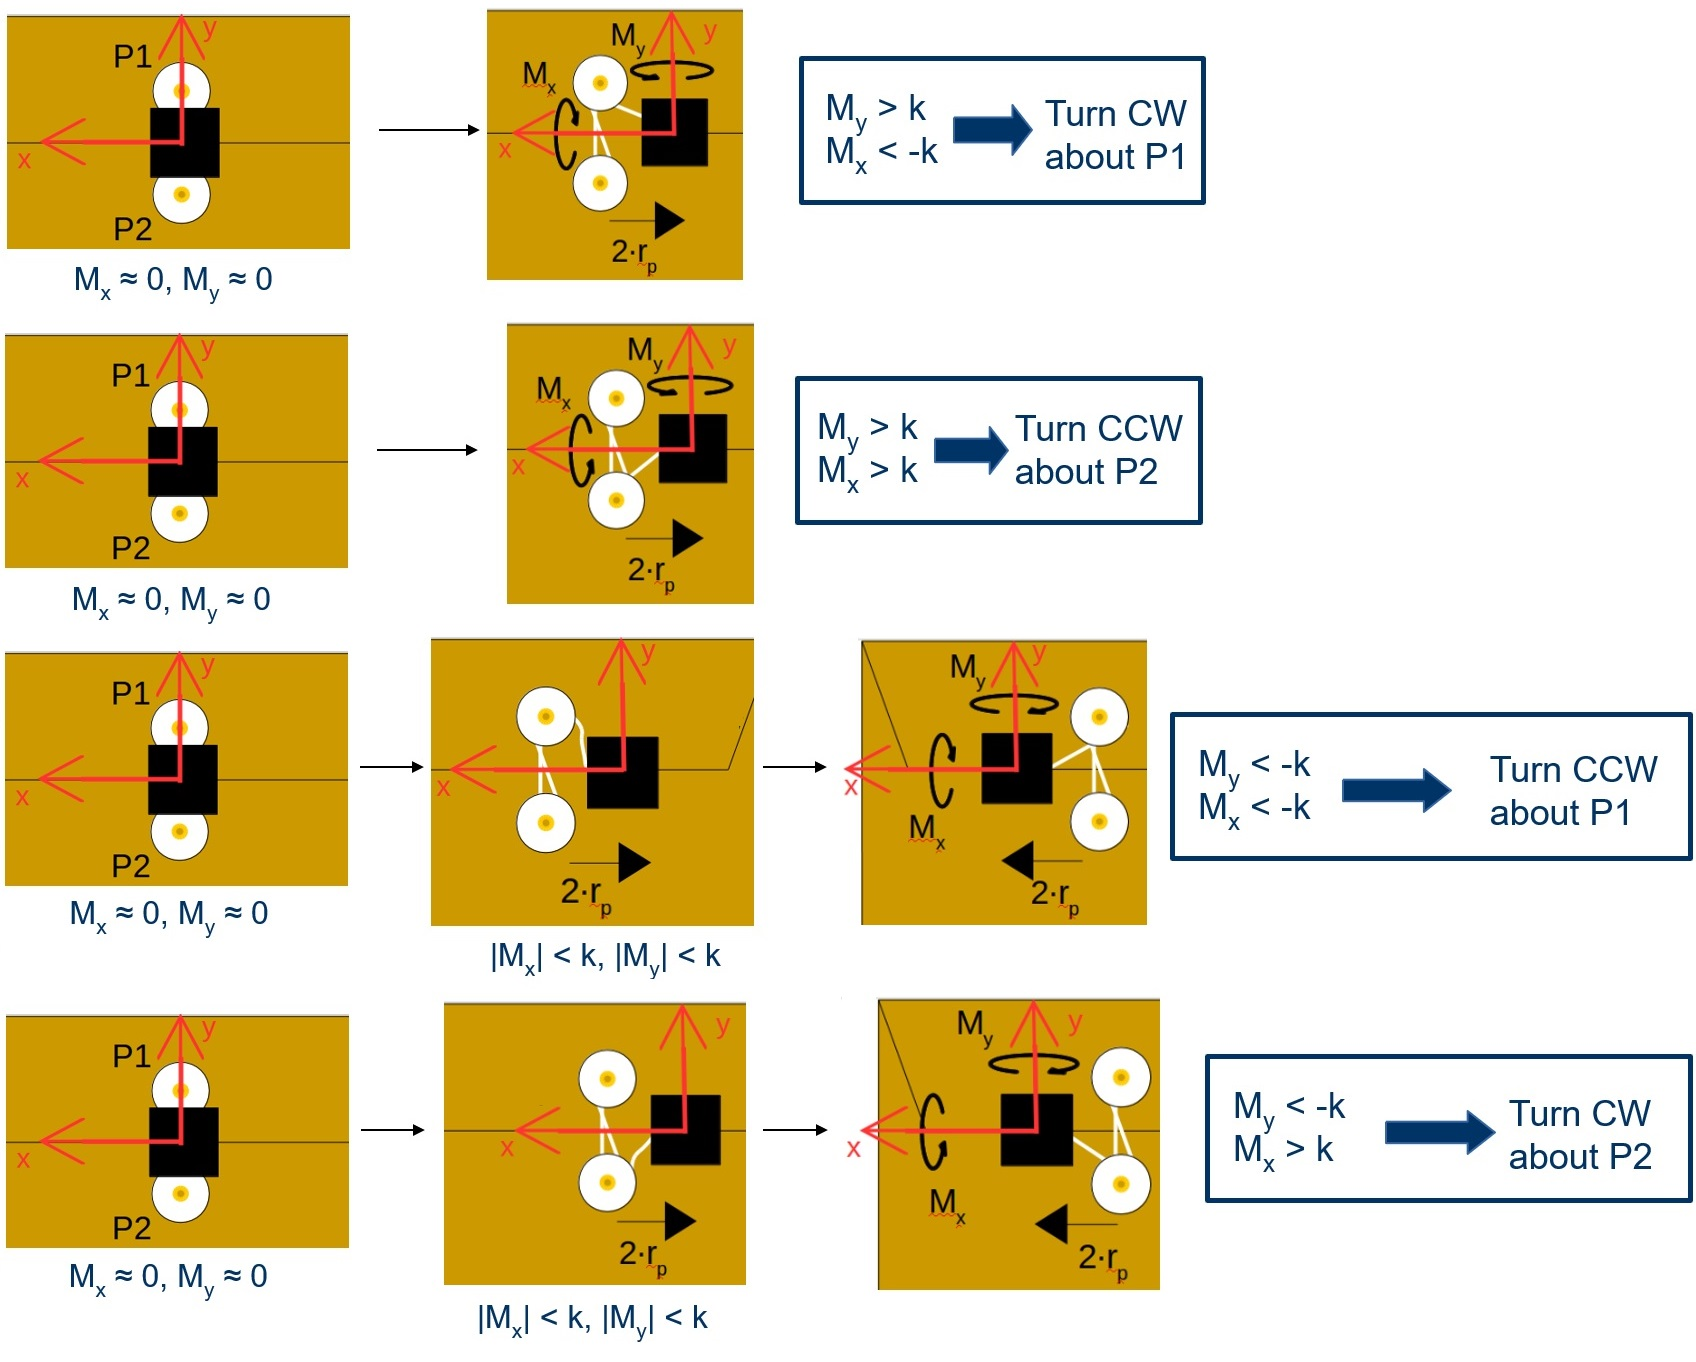
\includegraphics[height=130mm]{chapters/figures/algorithm/first_turn.jpg}
	\caption{Example of how the algorithm figures out the first turn.}
	\label{fig:first_turn}
\end{figure}

Let's tell the first turn was CW about P1, then Figure~\ref{fig:same_pivot} shows what happens after this turn if the string is again tied about the same pivot.
\begin{figure}[h!]
	\centering
	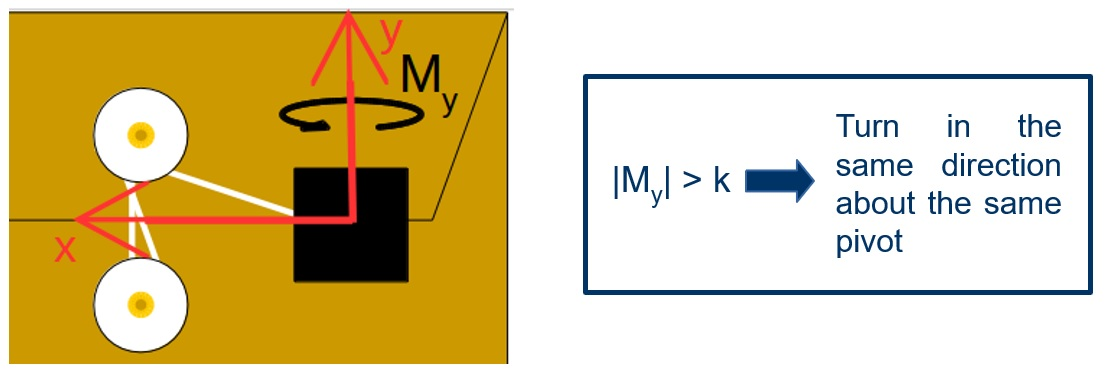
\includegraphics[height=40mm]{chapters/figures/algorithm/samepivot.jpg}
	\caption{Example of the case where the string is tied about the same pivot after one turn.}
	\label{fig:same_pivot}
\end{figure}

Otherwise, if the string is tied about the other pivot after the first turn, Figure~\ref{fig:other_pivot} shows what happens:
\begin{figure}[h!]
	\centering
	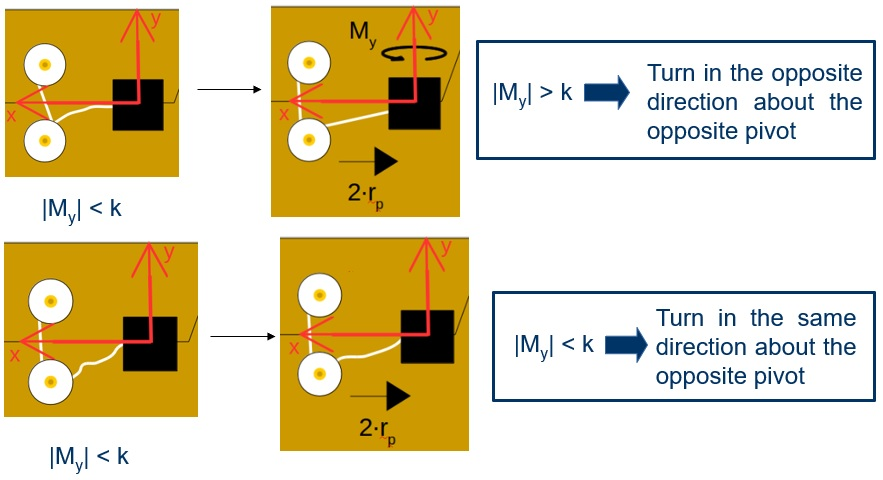
\includegraphics{chapters/figures/algorithm/otherpivot.jpg}
	\caption{Example of the cases where the string is tied about the other pivot after one turn.}
	\label{fig:other_pivot}
\end{figure}

 Finally, Figure~\ref{fig:end} shows how the algorithm figures out the end of the movement.
\begin{figure}[h!]
	\centering
	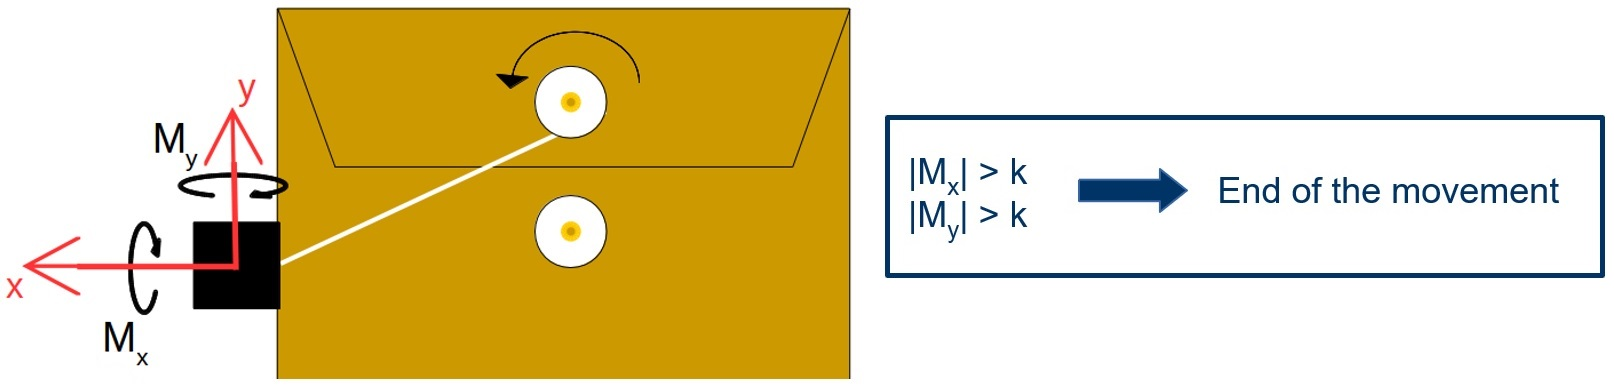
\includegraphics[height=40mm]{chapters/figures/algorithm/end.jpg}
	\caption{Example of the end of the movement.}
	\label{fig:end}
\end{figure}
\clearpage

%The word \textit{\textbf{robot}}\index{Robot} represents a very general concept that is hard to define precisely, since this word can be used to name a great amount of machines. 
%
%The aim of this chapter is to give an approximation to the concept of robot. Thus a brief history of robotics, the two technological roots of robotics, and finally an explanation to basic robotic jergon are presented.
%
%Let's start with a little riddle: which the following examples are robots?
%\begin{itemize}
% \item An automatic camera?
% \item An automatic washing machine?
% \item An automatic dishwasher?
% \item An automatic car (a car with an automatic gearbox)?
% \item A crane\footnote{gr\'ua}?
%\end{itemize}
%
%For some people, some or all of these examples are kinds of robots, for others none of them are. It all depends on what our own idea of what a robot is, and this can vary a lot from person to person.
%The word robot is often related with some kind of machine that has similarities to some part of human (or animal), body.  But this is not always true \ldots
%
%\section{A Little about the History}
%Although in appendix \ref{ch:introduntion} a review is made of remarkable milestones in \textit{\textbf{Robot history}} from the Ancient Greek culture to the present, let's see only the beginning of modern robotics. 
%
%The word robot was used for the first time in 1920 in a play entitled \textit{\textbf{R.U.R.}}\index{R.U.R} (\textit{\textbf{Rosum's Universal Robots}}\index{Rosum's Universal Robots}). This play was written by \textit{\textbf{Karel Capek}}\index{Karel Capek}, a Czech playwright. In the original Czeck, \textit{\textbf{Robota}}\index{Robota} means forced servitude. The name Rossum is an allusion to the Czech word rozum, which means reason, intellect. After the production of R.U.R. opened, the word robot displaced older words such as automaton or android in most languages. R.U.R stands for ''Rosumovi Um\v{e}l\'i Roboti'' (Mr. Reasson's Artificial Robots) and when the play was first put on in English-speaking countries, this title was translated from the Czech as ''Rossum's Universal Robots'' in order to fit the initials R.U.R (Figure~\ref{fig:rur}).
%
%\begin{figure}[htbp]
% \centering
% \includegraphics{chapters/figures/1_01_rur.jpg}
% \caption{A representation of a Rossum's Universal Robot.}
% \label{fig:rur}
%\end{figure}
% 
%In Capek's play, robots were human-like (humanoid) machines that were created by Rossum and his son to become servants of real human beings. But robots end up not accepting this role and rebel against humans. This resulted in a violent conflict between the people and the robots. However, it is the writer \textit{\textbf{Isaac Asimov}}\index{Isaac Asimov} to whom we owe the survival of the word robot. He is regarded as the father of Science Fiction Robots, since he was the first to refer to the science of robotics in a series of short stories that were collected in the book \textit{\textbf{I, Robot}}\index{I, Robot} (1950). 
%
%One of these stories is about a robot named Robbie \footnote{Text from the story Robbie that was first published as Strange Playfellow in Super Science Stories; 1940, Fictioners, Inc; 1968, Isaac Asimov}:
%\begin{quotation}
%Robbie was a non-vocal robot. He couldn't speak. He was made and sold in 1996. Those were the days before extreme specialization, so he was sold as a nursemaid.
%\begin{flushright} Dr Susan Calvin, U.S. Robotics, 2058\end{flushright}
%\end{quotation}
%
%In the story, Dr Calvin was an expert on robot-psychologists, and who was talking about the history of the company of the occasion of her retirement.
%
%The Asimov's vision is different from that of Capek. The latter envisages a pessimistic scenario for the relationship among humans and robots. The former defines in I, Robot robots as intelligent machines that have positronic brains. These positronic brains are programmed by humans, who stamp into them the \textit{\textbf{three laws of robotics}}\index{laws of robotics}, namely:
%\begin{description}
% \item [First Law]\index{laws of robotics, first} A robot must not harm a human being or, through inaction, allow one to come to harm;
% \item [Second Law]\index{laws of robotics,second} A robot must always obey human beings unless that is in conflict with the First Law;
% \item [Thrid Law]\index{laws of robotics, third} A robot must protect itself from harm unless that is in conflict with the First or Second Law.
%\end{description}
%
%Latter, the \textit{\textbf{Zeroth Law}}\index{laws of robotics, Zeroth}, was added: A robot may not injure humanity, or, through inaction, allow humanity to come to harm.
%
%Asimov's robot stories are a kind of exploration of the implications of implementing these laws in robots. However, the works of most other authors ignore or even contradict them. So, these laws have not prevailed as Asimov intended.
%
%Thus these three Laws are sometimes seen as a future design directives that should be considered by the people that would work in artificial intelligence, once an artificial intelligence has reached the stage where it can comprehend these laws. 
%
%\section {The Technological Roots of Robotics}
%The origins of robotics are linked to industrial robotics and can be traced in two separate, but related, technological developments.
%The first source came from the development of the \textit{\textbf{Computer Numerically Controlled Machine Tool}}\index{Computer Numerically Controlled Machine Tool} or \textit{\textbf{CNC Machine}}\index{CNC Machine}. The first CNC machine was developed at the MIT Servomechanisms Lab, USA, in 1952. It was the first programmable industrial machine tool.
%
%Secondly, working at the Aragonne National Labs, USA, \mbox{R. C. Goertz} demonstrated the first mechanical \textit{\textbf{telemanipulator}}\index{telemanipulator} (teleoperated device) in 1948 (Figure~\ref{fig:goertz}).  Seven years later, in 1954, he produced the first electric powered telemanipulator, which also had bilateral control. 
%
%The term \textit{\textbf{bilateral control}}\index{bilateral control} is used to define a kind of control  in which two robots are considered: the \textit{\textbf{master}}\index{Master robot} and the \textit{\textbf{slave robot}}\index{Slave robot}. The operator grasps and moves the master robot, and the slave robots tracks. But the interaction  forces/torques between the slave robot and its environment are also fed back to the master unit. This was a kind of haptic interface, of the sort that was later to be developed for more 'realistic' virtual reality systems.
%
%\begin{figure}[htbp]
% \centering
% \includegraphics[width=50mm]{chapters/figures/1_02_goertz.jpg}
% \caption{First teleoperated device. It was designed for radioactive material handling.}
% \label{fig:goertz}
%\end{figure}
%
%These two different technologies were subsequently combined in 1954, by \mbox{George C. Devol} in his \textit{\textbf{Programmable Object Transfer Device}}\index{Programmable Object Transfer Device}, a kind of programmable robot manipulator as the result of a combination of the electric telemanipulator and CNC control technologies.
%
%Then, in 1956, \mbox{George C. Devol} and \mbox{Joseph F. Engelberger} founded Consolidated Controls Corporation, which produced the first industrial robot to be installed in a General Motors factory in New Jersey. It was called the Unimate robot (universal automation robot). The name of the firm was later changed to Unimation Inc.. The Unimate was thus the first Industrial Robot, and Joseph Engelberger became know as the father of the Industrial Robot.
%
%\section{First Approach}
%A \textit{\textbf{robot}}\index{Robot} is a group of several \textit{\textbf{subsystems}}\index{Robot subsystems} each with its own function:
%\begin{description}
% \item [Mechanical system] By which the robot interacts with the surrounding environment. It usually performs one particular task. It consists of actuators, joints, wrists, tools, etc\ldots
% \item [Electrical system] Consisting of sensors, electrical/pneumatic/hydraulic actuators, computers, etc\ldots
% \item [Control system] This system receives high level orders and translates them into commands for actuators.
% \item [Sensor system] It measures different physical magnitudes so that control system is able to perform the correct action.
% \end{description}
% 
%The main feature for a robot is the availability of being reprogrammable. So it can be said that a robot is\ldots
%
%\begin{quotation}
%\ldots robot is a machine which can be programmed to do a variety of tasks, in the same way that a computer is an electronic circuit which can be programmed to do a variety of tasks.
%\begin{flushright}--Introduction to Robotics, Mac Kerrow\end{flushright} 
%\end{quotation}
%
%Another way of defining it is\ldots
%
%\begin{quotation}
%\ldots a computer-controlled mechanical device that can be programmed to do a variety of tasks without human supervision.
%\end{quotation}
%
%In this first approach, we will divide robots into three different categories: Science Fiction Robots, Toy Robots, and Real Robots. 
%
%\subsection{Science Fiction Robots}
%Since Robbie, in Asimov's story, there have been a lot more \textit{\textbf{Science Fiction robots}}: R2D2, C3P0 (Star Wars); HAL 9000 (2001: A Space Odissey); T1000 (Terminator), but to name a few (Figure~\ref{fig:fiction_robots}). The vast majority of these characters are baddies who typically act violently against people. In a sense, it is a little surprising that robots have been so often described as bad characters in Science Fiction stories.
%
%\begin{figure}[htbp]
% \centering
% \includegraphics[height=30mm]{chapters/figures/1_03_hal.jpg}
%\includegraphics[height=30mm]{chapters/figures/1_03_r2d2.jpg}
%\includegraphics[height=30mm]{chapters/figures/1_03_termi.jpg}
% \caption{Samples of Science Fiction Robots: HAL, R2D2, C3PO, T1000 (Terminator).}
% \label{fig:fiction_robots}
%\end{figure}
%
%Given that Since Science Fiction stories, films, and television programmes, are the source of most people's images and ideas about robots, it is hardly surprising that for many people robots are not bad or even frightening things. However, one of the possible answers to our question about what is a robot is precisely that a robot is a science fiction character. This is not the kind of robot we will consider in this course.
%
%\subsection{Toy Robots}
%As the second category, a robot could also be defined as a toy (Figure~\ref{fig:toy_robots}). There are many examples of \textit{\textbf{toy robots}}. Several of them are essentially models of science fiction robots, others are mere toys that we consider them as robots, or imitate life, for example Sony's Aibo pet robot dog.
%
%\begin{figure}[htbp]
% \centering
%\includegraphics[height=30mm]{chapters/figures/1_04_toy_bender.jpg}
%
% \caption{Samples of Toy Robots: Bender, R2D2.}
% \label{fig:toy_robots}
%\end{figure}
%
%Then, a question is arisen: when can a toy be thought as a robot? Not all toys that move around and make noises are robots. For most people, to be a robot, even a toy one, it is necessary to have arms, maybe legs, a head and eyes. In other words it is necessary to have a more or less humanoid form. This idea, the humanoid form, is important, and comes from the images of science fiction robots, most of which are also humanoid. Therefore, robots can be also toys, and they normally have a humanoid form.
%
%\subsection{Real Robots}
%The last category groups the robots that operate in the real world. They can be further subdivided into four different types:
%\begin{description}
% \item [Industrial robot] these are the vast majority of existing robots;
% \item [Service robots] there are hardly any yet;
% \item [Biomedical robot] a quite new and promising application field to robotics;
% \item [Experimental or Scientific robots] the second most popular type of real robot.
%\end{description}
%
%
% 
%
%\begin{table}[!ht]
%
%\centering
%		\begin{tabular}{ccc} 
%		\hline
%		\textbf{Feature}&\textbf{Omni}&\textbf{Premium 1.5}\\\hline
%		Sensed Degree of Freedom (DoF) & 6 & 6\\
%		Actuated Degree of Freedom (DoF) & 3 & 6\\
%		Workspace&16x12x7 cm& 38x26x19cm\\
%		Accuracy (translation)& 0.055mm & 0.03mm\\
%		Maximum Force (peak) & 3.3 N& 8.5 N\\
%		Maximum Force (continuous) & 0.88 N & 1.4 N\\
%		Apparent inertia & 45 g & 136 g\\\hline
%			
%		\end{tabular}
%\caption{Mechanical features of two PHANToM haptic devices.}
%\label{table:tomni}
%\end{table}
%
%
%
%\begin{equation}
% q=
%\begin{bmatrix}
% q_{1} & q_{2} & \ldots &q_{n}\\
%\end{bmatrix} ^{T}
%\end{equation}
%
%where n is the number of degrees of freedom.
%
%Usually industrial robot arms have between 4 and 6 degrees of freedom, one at each joint.
%
%\subsection{End Point}
%It is the point of the mechanism/manipulator that we want to place in a specific location. Mathematically, we will define the end-point as $p_e$. It is also where the robot's end-effector (the gripper or the tool) is attached. Seg\'un ecuaci\'on \ref{eq:miEcuacion}
%
%\begin{equation}
%p_e=
%\begin{bmatrix}
%p_{x_e}&p_{y_e}&p_{z_e} \\
%\end{bmatrix}^{T}
%\label{eq:miEcuacion}
%\end{equation}
%
%
%$
%p_e=
%\begin{bmatrix}
%p_{x_e}&p_{y_e}&p_{z_e} \\
%\end{bmatrix}^{T}
%$
%
%
%If, for example, the robot has a two-finger \textit{\textbf{gripper}}, to pick things up with, we usually define $p_e$ to be a point between the two \textit{\textbf{fingers}} (when they are open), so that when this point is geometrically inside some object to be picked up, all the robot has to do is to close the fingers of its gripper to grasp the object. It can then move away with the object between its fingers.
%
%It is not sufficient for $P_e$ just to be defined as a point. We also need to attach or (conceptually) fix a coordinate system to it, so that we can define both the position of $p_e$ in space, and its orientation ($\psi_e$). In this way we are able to define the position and orientation of the robot's gripper in terms of the position and orientation of $P_e$. 
%
%\begin{equation}
%P_e=
%\begin{bmatrix}
%p_e\\\mathit{\psi}_e
%\end{bmatrix}
%=
%\begin{bmatrix} 
%&\text{position}&\\ \cline{2-2}  &\text{orientation}&
%\end{bmatrix}
%\end{equation}
%
%\subsection{Cartesian Space vs. Joint Space}\index{Cartesian space}\index{Join space}
%The robot's \textit{\textbf{end-point}} can be determined by the values of the joint positions of the arm ($q_1$, $q_2$, $q_3$, etc.) and the geometry of the elements of the robot arm that connect each pair of joints. Then we say that the robot's end point is defined in the joint space.
%
%The position and orientation of the end point can also be defined with respect to some global Cartesian frame of reference, some global coordinate system. For this, we usually use a frame of reference fixed to the base of the robot, which should not move. Thus, we determine the position and orientation of the end-point in the Cartesian space.
%
%Any particular position and orientation of $P_e$ in space, and so any particular set of joint values, is called a \textit{\textbf{configuration of the robot arm}}\index{Configuration of the robot arm}.
%
%\subsection{Workspace}\index{Workspace}
%It is the locus that contains the reachable space by the robot's end-point. But this is different from \textit{\textbf{workspace envelope}}\index{Workspace envelope}. 
%The \textit{\textbf{workspace limitations}}\index{Workspace limitation}:
%\begin{itemize}
% \item Actuators endstroke.
% \item Working range of joints.
% \item Collisions among manipulator's link.
%\end{itemize}
%
%We can define the robot workspace in two ways:
%
%\begin{enumerate}
%	\item The {\CPRindex{Dextrous Workspace}}, $WS_D$, is the volume of the theoretical workspace in which $P_e$ can be oriented in any way.
%	\item The {\CPRindex{Reachable Workspace}}, $WS_R$, is the volume of the theoretical workspace to which $P_e$ can be moved in at least one orientation.
%\end{enumerate}
%
%Clearly $WS_D$ is a subset (sub-volume) of $WS_R$.
%
%It is also desirable that both $WS_D$ and $WS_R$ have no `holes' in them, internal sub-volumes that are not reachable by $P_e$.
%


\chapter{EXPERIMENTAL RESULTS}
\label{ch:Experimental Results}
In this chapter we show the experiments we have made and their results.

The four experiments we talk about here are the following:
\begin{itemize}
 \item Experiment 1: Why use torque values instead of force.
 \item Experiment 2: Minimum radius of the pivot.
 \item Experiment 3: Minimum distance between pivots.
 \item Experiment 4: Comparison of robot fail ratio with human fail ratio.
\end{itemize}

The first experiment explains why we used torque values in this work instead of force values to determine the direction of string tension. We also explain how the threshold value for torque has been established.

The second experiment shows which is the minimum radius for the pivot to distinguish between CW and CCW case. We establish the minimum radius from which the pivot is considered negligible.

The third experiment consists on establishing the minimum distance between pivots to distinguish them through torque values.

Finally, the fourth experiment consists on comparing robot fail ratio with human fail ratio. There we do several experiments with the robot, and then we repeat the same experiments with different people in the same conditions than the robot (with no vision).

Let's start explaining the first experiment.

\section{Experiment 1: Why use torque values instead of force}
As told before, here we explain why we use torques instead of forces and then we establish the threshold from which torque values are considered relevant.

\subsection{Comparison between force values and torque values}
It is true that the most intuitive way to solve the problem of untying the string from the pivot would be to look at forces because these would directly tell the direction of string tension. But, let's see what happens if we look to force and torque readings of the Robotiq FT300 sensor in the case where there is no tension of the string and in the case where there is.

For this experiment, the case of no string tension is the initial pose, when the gripper is just grasping the end of the string between the two pivots, before starting the movement. The case of string tension is the case when the gripper moves $2 \cdot r_{p}$ in perpendicular to pivots joining axis. Figure~\ref{fig:exp1} below shows both cases.
\begin{figure}[h!]
	\centering
	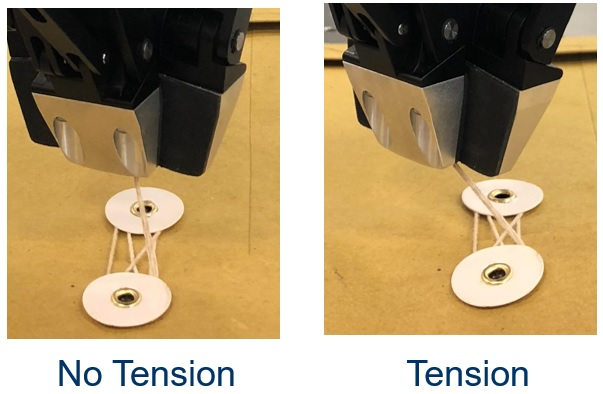
\includegraphics[height=60mm]{chapters/figures/experiments/exp1.jpg}
	\caption{Tension and No Tension cases.}
	\label{fig:exp1}
\end{figure}

Let's take 30 values of force and torque from the force/torque sensor in both cases. Results are presented in Table~\ref{tab:readings}.%\clearpage
% Table generated by Excel2LaTeX from sheet 'CW P1'
%\begin{longtable}[htbp]
%\begin{center}
\setlength\LTpost{0pt}
\begin{longtable}{|c|c|c|c|rr|c|c|c|c|}
		\cmidrule{1-4}\cmidrule{7-10}    \multicolumn{4}{|c|}{\textbf{NO TENSION (INITIAL POSE)}} &       &       & \multicolumn{4}{c|}{\textbf{TENSION (CW P1)}} \\
		\cmidrule{1-4}\cmidrule{7-10}    \textbf{$F_{x} (N)$} & \textbf{$F_{y} (N)$} & \textbf{$M_{x} (N \cdot m)$} & \textbf{$M_{y} (N \cdot m)$} &       &       & \textbf{$F_{x} (N)$} & \textbf{$F_{y} (N)$} & \textbf{$M_{x} (N \cdot m)$} & \textbf{$M_{y} (N \cdot m)$} \\
		\cmidrule{1-4}\cmidrule{7-10}    1.19  & 1.41  & 0.072 & 0.032 &       &       & 2.55  & -0.04 & -0.177 & 0.422 \\
		0.76  & 0.27  & 0.023 & 0.035 &       &       & 2.81  & 1.56  & -0.199 & 0.431 \\
		-0.04 & -0.19 & 0.060 & 0.007 &       &       & 2.25  & -0.40 & -0.194 & 0.432 \\
		0.13  & -1.28 & 0.057 & 0.006 &       &       & 2.34  & 0.06  & -0.170 & 0.412 \\
		1.96  & 0.13  & 0.056 & 0.030 &       &       & 3.31  & -1.18 & -0.184 & 0.422 \\
		0.71  & -0.63 & 0.033 & 0.037 &       &       & 3.75  & 1.00  & -0.215 & 0.440 \\
		1.61  & -0.26 & 0.043 & 0.045 &       &       & 2.71  & 1.00  & -0.214 & 0.446 \\
		1.79  & -0.90 & 0.056 & 0.010 &       &       & 3.96  & 1.24  & -0.214 & 0.434 \\
		0.13  & 0.28  & 0.049 & 0.039 &       &       & 3.28  & 2.52  & -0.190 & 0.411 \\
		-0.65 & 0.31  & 0.009 & 0.044 &       &       & 5.23  & -0.31 & -0.196 & 0.448 \\
		-0.88 & -0.81 & 0.063 & 0.045 &       &       & 2.18  & -0.44 & -0.212 & 0.425 \\
		-0.36 & 1.10  & 0.069 & 0.014 &       &       & 3.60  & 1.04  & -0.198 & 0.411 \\
		0.43  & -0.49 & 0.056 & 0.049 &       &       & 3.47  & 2.06  & -0.191 & 0.406 \\
		-0.64 & -0.10 & 0.065 & 0.029 &       &       & 2.41  & 0.46  & -0.157 & 0.430 \\
		0.50  & -0.22 & 0.058 & 0.032 &       &       & 3.65  & 1.72  & -0.169 & 0.416 \\
		-0.42 & -0.89 & 0.067 & 0.031 &       &       & 3.04  & -0.91 & -0.191 & 0.409 \\
		0.15  & -1.66 & 0.074 & 0.020 &       &       & 3.23  & 0.08  & -0.177 & 0.403 \\
		-0.74 & 0.89  & 0.074 & 0.028 &       &       & 3.18  & 1.10  & -0.190 & 0.415 \\
		1.38  & -1.86 & 0.071 & 0.037 &       &       & 4.07  & 0.63  & -0.192 & 0.407 \\
		0.21  & -1.05 & 0.073 & 0.048 &       &       & 4.28  & -0.57 & -0.197 & 0.428 \\
		0.26  & -0.95 & 0.072 & 0.022 &       &       & 3.86  & 0.14  & -0.207 & 0.390 \\
		0.38  & -1.54 & 0.061 & 0.035 &       &       & 3.26  & -1.17 & -0.188 & 0.442 \\
		1.43  & -2.17 & 0.058 & 0.057 &       &       & 3.17  & 0.10  & -0.199 & 0.368 \\
		0.16  & -0.71 & 0.013 & 0.058 &       &       & 3.05  & 0.06  & -0.173 & 0.438 \\
		-0.67 & -0.21 & 0.078 & 0.045 &       &       & 4.87  & 1.35  & -0.182 & 0.444 \\
		0.21  & -1.97 & 0.065 & 0.021 &       &       & 2.30  & 0.67  & -0.155 & 0.403 \\
		0.06  & -0.46 & 0.063 & 0.001 &       &       & 3.23  & 3.23  & -0.200 & 0.409 \\
		1.43  & -1.37 & 0.044 & 0.026 &       &       & 4.64  & -0.95 & -0.180 & 0.417 \\
		-1.43 & -0.77 & 0.042 & 0.049 &       &       & 3.67  & 2.00  & -0.171 & 0.407 \\
		1.08  & -0.83 & 0.073 & 0.015 &       &       & 1.12  & -0.19 & -0.199 & 0.430 \\
		\cmidrule{1-4}\cmidrule{7-10}    %\end{longtable}%
	\caption{Results of force and torque readings for the case of no tension and the case of tension of the string.}
	\label{tab:readings}%
\end{longtable}% 
%\end{center}% 

Now let's look to the maximum and minimum values in each case (Table~\ref{tab:maxmin}).
% Table generated by Excel2LaTeX from sheet 'CW P1'
% Table generated by Excel2LaTeX from sheet 'CW P1'
\begin{table}[htbp]
	\centering
	\begin{tabular}{l|c|c|c|c|c|c|c|c|}
		\cmidrule{2-9}
		& \multicolumn{4}{c|}{\textbf{NO TENSION (INITIAL POSE)}} & \multicolumn{4}{c|}{\textbf{TENSION (CW P1)}} \\
		\cmidrule{2-9}
		\multicolumn{1}{r|}{} & \textbf{$F_{x} (N)$} & \textbf{$F_{y} (N)$} & \textbf{$M_{x} (N \cdot m)$} & \textbf{$M_{y} (N \cdot m)$} & \textbf{$F_{x} (N)$} & \textbf{$F_{y} (N)$} & \textbf{$M_{x} (N \cdot m)$} & \textbf{$M_{y} (N \cdot m)$} \\
		\midrule
		\multicolumn{1}{|l|}{\textbf{Min}} & -1.43 & -2.17 & 0.009 & 0.001 & 1.12  & -1.18 & -0.215 & 0.368 \\
		\midrule
		\multicolumn{1}{|l|}{\textbf{Max}} & 1.96  & 1.41  & 0.078 & 0.058 & 5.23  & 3.23  & -0.155 & 0.448 \\
		\midrule
		\multicolumn{1}{|l|}{\textbf{Max - Min}} & 3.39  & 3.58  & 0.069 & 0.057 & 4.11  & 4.41  & 0.060 & 0.080 \\
		\bottomrule
	\end{tabular}%
	\caption{Maximum and minimum values of force and torque.}
	\label{tab:maxmin}%
\end{table}%

We appreciate that the difference between the maximum and the minimum value for force readings is around $4 N$, while for torques it is around $0.070 N \cdot m$. The sensor is much noisier for force readings than for torques. Furthermore, if we compare maximum and minimum values in \textit{tension} and \textit{no tension} case, we see that force values are overlapped in both cases:
\[ F_{x, max, no tension} = 1.96 N > 1.12 N = F_{x, min, tension} \]
\[ F_{y, max, no tension} = 1.41 N > -1.18 N = F_{y, min, tension} \]

While torques are clearly distinguishable:
\[ M_{x, min, no tension} = 0.009 N\cdot m > -0.155 N\cdot m = M_{x, max, tension} \]
\[ M_{y, max, no tension} = 0.058 N\cdot m < 0.368 N\cdot m = M_{y, min, tension} \]

As there is an error in sensor readings, we decided to take the mean values as the most accurates values to compare both cases. Let's look now to mean values and standard deviation in Table~\ref{tab:mean}.
% Table generated by Excel2LaTeX from sheet 'CW P1'
%\begin{table}[htbp]
%	\centering
%	\begin{tabular}{|l|c|c|c|c|c|}
\setlength\LTpost{0pt}
\begin{longtable}{|l|c|c|c|c|c|}
		\multicolumn{1}{|r}{} &       & \textbf{$F_{x} (N)$} & \textbf{$F_{y} (N)$} & \textbf{$M_{x} (N \cdot m)$} & \textbf{$M_{y} (N \cdot m)$} \\
		\midrule
		\multicolumn{1}{|p{9.125em}|}{\textbf{NO TENSION}} & St. dev. & 0.86  & 0.89  & 0.018  & 0.015 \\
		\cmidrule{2-6}    \textbf{(INITIAL POSE)} & Mean  & 0.34  & -0.56 & 0.057  & 0.032 \\
		\midrule
		\multicolumn{1}{|p{9.125em}|}{\textbf{TENSION}} & St. dev. & 0.87  & 1.12  & 0.016  & 0.018 \\
		\cmidrule{2-6}    \textbf{(CW P1)} & Mean  & 0.49  & 0.53  & -0.189 & 0.42 \\
		\bottomrule
%	\end{tabular}%
	\caption{Standard deviation and mean values for force and torque readings in tension and no tension case.}
	\label{tab:mean}%
\end{longtable}%

With this values of standard deviation and mean, we establish the ranges of force and torque variations for tension and no tension case. The results are shown in Table~\ref{tab:ranges}.
% Table generated by Excel2LaTeX from sheet 'CW P1'
%\begin{table}[htbp]
%	\centering
%	\setlength\LTpre{0pt}
\setlength\LTpost{0pt}
\begin{longtable}{|c|c|c|}
		\cmidrule{2-3}    \multicolumn{1}{c|}{} & \multicolumn{1}{p{12.915em}|}{\textbf{No Tension (Initial pose)}} & \multicolumn{1}{p{12.915em}|}{\textbf{Tension case (CW P1)}} \\
		\midrule
		\textbf{$F_{x} \pm st. dev. (N)$} & $-0.52 N < F_{x} < 1.2 N$ & $-0.38 N < F_{x} < 1.36 N$ \\
		\midrule
		\textbf{$F_{y} \pm st. dev. (N)$} & $-1.45 N < F_{y} < 0.33 N$ & $-0.59 N < F_{y} < 1.65 N$ \\
		\midrule
		\textbf{$M_{x} \pm st. dev. (N \cdot m)$} & $0.039 N \cdot m < M_{x} < 0.075 N \cdot m$ & $-0.205 N \dot m < M_{x} < -0.173 N \cdot m$ \\
		\midrule
		\textbf{$M_{y} \pm st. dev. (N \cdot m)$} & $0.017 N \cdot m < M_{y} < 0.047 N \cdot m$ & $0.402 N \cdot m < M_{y} < 0.438 N \cdot m$ \\
		\bottomrule
%	\end{longtable}%
	\caption{Ranges of force and torque variations in tension and no tension cases.}
	\label{tab:ranges}%
\end{longtable}%

Looking to forces values, we see that both ranges for $F_{x}$ and $F_{y}$ are overlapped in case of tension and no tension. Variation in force readings is too big compared to the little forces (tension of the string) we are working with. We can thus not distinguish between the tension case and no tension case with force values. Force cannot be used to determine the direction of string tension in this case.

Otherwise, if we look to torque values, we see that ranges for tension case and no tension case are clearly distinguishable. Torque readings are much more precise than force readings and that is why we use torque values in this work.

\subsection{Threshold value for torque}
After explaining why torque values are more accurate for this project, let's establish now the threshold value for torque readings to be considered relevant. 

To  do that, we made 10 experiments where we took 30 values of torque in tension and in no tension case. Then, with the mean and the standard deviation we compare both cases of each experiment. We show directly the results for the mean and standard deviation in each experiment. These are shown in Table~\ref{tab:experimenttorques} below:
% Table generated by Excel2LaTeX from sheet 'CW P1'
\setlength\LTpost{0pt}
\begin{longtable}{|r|c|c|c|c|c|}
		\cmidrule{3-6}    \multicolumn{1}{r}{} &       & \multicolumn{2}{c|}{\textbf{NO TENSION (INITIAL POSE)}} & \multicolumn{2}{c|}{\textbf{TENSION (CW P1)}} \\
		\cmidrule{3-6}    \multicolumn{1}{r}{} &       & \textbf{St. dev.} & \textbf{Mean} & \textbf{St. dev.} & \textbf{Mean} \\
		\midrule
		\multicolumn{1}{|l|}{\textbf{Experiment 1}} & \textbf{$M_{x} (N \cdot m)$} & 0.018 & 0.057 & 0.016 & -0.189 \\
		\cmidrule{2-6}          & \textbf{$M_{y} (N \cdot m)$} & 0.015 & 0.032 & 0.018 & 0.42 \\
		\midrule
		\multicolumn{1}{|l|}{\textbf{Experiment 2}} & \textbf{$M_{x} (N \cdot m)$} & 0.022 & 0.042 & 0.021 & -0.168 \\
		\cmidrule{2-6}          & \textbf{$M_{y} (N \cdot m)$} & 0.016 & 0.033 & 0.026 & 0.140 \\
		\midrule
		\multicolumn{1}{|l|}{\textbf{Experiment 3}} & \textbf{$M_{x} (N \cdot m)$} & 0.017 & 0.028 & 0.024 & -0.072 \\
		\cmidrule{2-6}          & \textbf{$M_{y} (N \cdot m)$} & 0.024 & 0.042 & 0.022 & 0.184 \\
		\midrule
		\multicolumn{1}{|l|}{\textbf{Experiment 4}} & \textbf{$M_{x} (N \cdot m)$} & 0.019 & 0.052 & 0.024 & -0.056 \\
		\cmidrule{2-6}          & \textbf{$M_{y} (N \cdot m)$} & 0.014 & 0.047 & 0.015 & 0.143 \\
		\midrule
		\multicolumn{1}{|l|}{\textbf{Experiment 5}} & \textbf{$M_{x} (N \cdot m)$} & 0.015 & 0.031 & 0.018 & -0.173 \\
		\cmidrule{2-6}          & \textbf{$M_{y} (N \cdot m)$} & 0.022 & 0.022 & 0.019 & 0.215 \\
		\midrule
		\multicolumn{1}{|l|}{\textbf{Experiment 6}} & \textbf{$M_{x} (N \cdot m)$} & 0.016 & 0.009 & 0.024 & -0.240 \\
		\cmidrule{2-6}          & \textbf{$M_{y} (N \cdot m)$} & 0.015 & 0.020 & 0.016 & 0.199 \\
		\cmidrule{1-1}\cmidrule{3-6}    \multicolumn{1}{|l|}{\textbf{Experiment 7}} & \textbf{$M_{x} (N \cdot m)$} & 0.021 & 0.053 & 0.020 & -0.291 \\
		\cmidrule{2-6}          & \textbf{$M_{y} (N \cdot m)$} & 0.028 & 0.045 & 0.023 & 0.284 \\
		\midrule
		\multicolumn{1}{|l|}{\textbf{Experiment 8}} & \textbf{$M_{x} (N \cdot m)$} & 0.028 & 0.055 & 0.016 & -0.078 \\
		\cmidrule{2-6}          & \textbf{$M_{y} (N \cdot m)$} & 0.021 & 0.031 & 0.011 & 0.152 \\
		\midrule
		\multicolumn{1}{|l|}{\textbf{Experiment 9}} & \textbf{$M_{x} (N \cdot m)$} & 0.026 & 0.038 & 0.018 & -0.085 \\
		\cmidrule{2-6}          & \textbf{$M_{y} (N \cdot m)$} & 0.015 & 0.017 & 0.021 & 0.141 \\
		\midrule
		\multicolumn{1}{|l|}{\textbf{Experiment 10}} & \textbf{$M_{x} (N \cdot m)$} & 0.023 & 0.053 & 0.021 & -0.115 \\
		\cmidrule{2-6}          & \textbf{$M_{y} (N \cdot m)$} & 0.027 & 0.056 & 0.018 & 0.202 \\
		\bottomrule
		\caption{Results for 10 experiments of standard deviation and mean values for torque in tension and no tension case.}
		\label{tab:experimenttorques}%
\end{longtable}%

The maximum value of standard deviation is $0.028 N\cdot m$ in experiments 7 and 8, so the threshold value must be greater than $0.028 N\cdot m$. 

To see if any torque value is overlapped in tension and no tension case, let's establish the ranges of variation of torque in each experiment. These ranges are shown in  Table~\ref{tab:rangetorques}:
% Table generated by Excel2LaTeX from sheet 'CW P1'
\setlength\LTpost{0pt}
\begin{longtable} {|r|c|c|c|c|c|}
		\cmidrule{3-4}    \multicolumn{1}{r}{} &       & \textbf{NO TENSION (INITIAL POSE)} & \textbf{TENSION (CW P1)} \\
		\midrule
		\multicolumn{1}{|l|}{\textbf{Exp. 1}} & \textbf{$M_{x} \pm st. dev. (N \cdot m)$} & $0.039 < M_{x} < 0.075$ & $-0.205 < M_{x} < -0.173 $ \\
		& \textbf{$M_{y} \pm st. dev. (N \cdot m)$} & $0.017 < M_{y} < 0.047$ & $0.402 < M_{y} < 0.438$ \\
		\cmidrule{1-4}
		\multicolumn{1}{|l|}{\textbf{Exp. 2}} & \textbf{$M_{x} \pm st. dev. (N \cdot m)$} & $0.02 < M_{x} < 0.064$ & $-0.189 < M_{x} < -0.147$ \\
		& \textbf{$M_{y} \pm st. dev. (N \cdot m)$} & $0.017 < M_{y} < 0.049$ & $0.114 < M_{y} < 0.166$ \\
		\cmidrule{1-4}
		\multicolumn{1}{|l|}{\textbf{Exp. 3}} & \textbf{$M_{x} \pm st. dev. (N \cdot m)$} & $0.011 < M_{x} < 0.045$ & $-0.096 < M_{x} < -0.048$ \\
		& \textbf{$M_{y} \pm st. dev. (N \cdot m)$} & $0.018 < M_{y} < 0.066$ & $0.162 < M_{y} < 0.206$ \\
		\cmidrule{1-4}
		\multicolumn{1}{|l|}{\textbf{Exp. 4}} & \textbf{$M_{x} \pm st. dev. (N \cdot m)$} & $0.033 < M_{x} < 0.071$ & $-0.08 < M_{x} < -0.032$ \\
		& \textbf{$M_{y} \pm st. dev. (N \cdot m)$} & $0.033 < M_{y} < 0.061$ & $0.128 < M_{y} < 0.158$ \\
		\cmidrule{1-4}
		\multicolumn{1}{|l|}{\textbf{Exp. 5}} & \textbf{$M_{x} \pm st. dev. (N \cdot m)$} & $0.016 < M_{x} < 0.046$ & $-0.191 < M_{x} < -0.155$ \\
		& \textbf{$M_{y} \pm st. dev. (N \cdot m)$} & $0.000 < M_{y} < 0.044$ & $0.196 < M_{y} < 0.234$ \\
		\cmidrule{1-4}
		\multicolumn{1}{|l|}{\textbf{Exp. 6}} & \textbf{$M_{x} \pm st. dev. (N \cdot m)$} & $-0.007 < M_{x} < 0.025$ & $-0.264 < M_{x} < -0.216$ \\
		& \textbf{$M_{y} \pm st. dev. (N \cdot m)$} & $0.005 < M_{y} < 0.035$ & $0.183 < M_{y} < 0.215$ \\
		\cmidrule{1-4}
		\multicolumn{1}{|l|}{\textbf{Exp. 7}} & \textbf{$M_{x} \pm st. dev. (N \cdot m)$} & $0.032 < M_{x} < 0.074$ & $-0.311 < M_{x} < -0.271$ \\
		& \textbf{$M_{y} \pm st. dev. (N \cdot m)$} & $0.017 < M_{y} < 0.073$ & $0.261 < M_{y} < 0.307$ \\
		\cmidrule{1-4}
		\multicolumn{1}{|l|}{\textbf{Exp. 8}} & \textbf{$M_{x} \pm st. dev. (N \cdot m)$} & $0.027 < M_{x} < 0.083$ & $-0.094 < M_{x} < -0.062$ \\
		& \textbf{$M_{y} \pm st. dev. (N \cdot m)$} & $0.010 < M_{y} < 0.052$ & $0.141 < M_{y} < 0.163$ \\
		\cmidrule{1-4}
		\multicolumn{1}{|l|}{\textbf{Exp. 9}} & \textbf{$M_{x} \pm st. dev. (N \cdot m)$} & $0.012 < M_{x} < 0.064$ & $-0.103 < M_{x} < -0.067$ \\
		& \textbf{$M_{y} \pm st. dev. (N \cdot m)$} & $0.002 < M_{y} < 0.032$ & $0.120 < M_{y} < 0.162$ \\
		\cmidrule{1-4}
		\multicolumn{1}{|l|}{\textbf{Exp. 10}} & \textbf{$M_{x} \pm st. dev. (N \cdot m)$} & $0.030 < M_{x} < 0.076$ & $-0.136 < M_{x} < -0.094$ \\
		& \textbf{$M_{y} \pm st. dev. (N \cdot m)$} & $0.029 < M_{y} < 0.083$ & $0.184 < M_{y} < 0.220$ \\
		\bottomrule
	\caption{Range of variation of torques in 10 experiments.}
	\label{tab:rangetorques}%
\end{longtable}%

We appreciate that in the 10 experiments, ranges in tension case and in no tension case are never overlapped. 

Finally, we look to the difference between the means of both cases in each experiment (Table~\ref{tab:meandifference}).
% Table generated by Excel2LaTeX from sheet 'CW P1'
\begin{table}[htbp]
	\centering
	\begin{tabular}{|l|c|c|}
		\cmidrule{2-3}    \multicolumn{1}{r|}{} & \textbf{$M_{x, tension} - M_{x, no tension} (N \cdot m)$} & \textbf{$M_{y, tension} - M_{y, no tension} (N \cdot m)$} \\
		\midrule 
		\textbf{Experiment 1} & -0.246 & 0.388 \\
		\midrule
		\textbf{Experiment 2} & -0.21 & 0.107 \\
		\midrule
		\textbf{Experiment 3} & -0.100 & 0.142 \\
		\midrule
		\textbf{Experiment 4} & -0.108 & 0.096 \\
		\midrule
		\textbf{Experiment 5} & -0.204 & 0.193 \\
		\midrule
		\textbf{Experiment 6} & -0.249 & 0.179 \\
		\midrule
		\textbf{Experiment 7} & -0.344 & 0.239 \\
		\midrule
		\textbf{Experiment 8} & -0.133 & 0.121 \\
		\midrule
		\textbf{Experiment 9} & -0.123 & 0.124 \\
		\midrule
		\textbf{Experiment 10} & -0.168 & 0.146 \\
		\bottomrule
	\end{tabular}%
	\caption{Difference between means in tension and no tension case for 10 experiments.}
	\label{tab:meandifference}%
\end{table}%

We appreciate that the minimum difference between the 2 cases is for $M_{y}$ in experiment 4, and the value is $0.096 N \cdot m$. We decided thus, to establish a threshold value of \textbf{$0.095 N \cdot m$} from which we consider that the string is taut. Furthermore, this value is greater than $0.028 N\cdot m$, which is the maximum standard deviation. 

\section{Experiment 2: Minimum radius of the pivots}
In this section we show the experiment made to figure out which is the minimum radius of the pivots for the sensor to distinguish between CW and CCW case.

For this, we took different objects with different radius and we wound the thread around them. By moving $2 \cdot r_{p}$, we see when torque values do not allow to distinguish anymore between CW and CCW case.

\subsection{Radius = 4 mm}
We start with the real radius of our pivots. This is 4 mm. In Figure~\ref{fig:CWCCW1} below, we can see the difference between CW and CCW case:
\begin{figure}[h!]
	\centering
	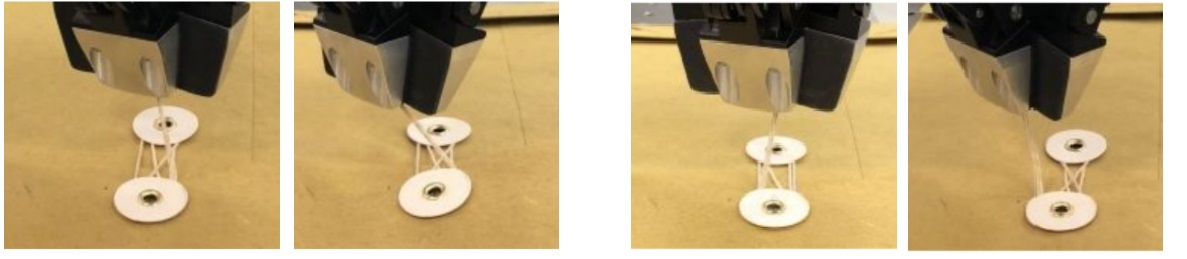
\includegraphics[height=35mm]{chapters/figures/experiments/exp2_CWCCW1.jpg}
	\caption{CW case on the left and CCW case on the right for r = 4 mm.}
	\label{fig:CWCCW1}
\end{figure}

Let's see the results for torques in Table~\ref{tab:4mm}.
% Table generated by Excel2LaTeX from sheet 'CW P1'
\begin{table}[htbp]
	\centering
	\begin{tabular}{|l|c|c|c|}
		\cmidrule{2-4}    \multicolumn{1}{r|}{} & \multicolumn{3}{c|}{\textbf{r = 4 mm}} \\
		\cmidrule{2-4}    \multicolumn{1}{r|}{} & \textbf{$|M_{x, tension} - M_{x, no tension}|$} & \textbf{$|M_{y, tension} - M_{y, no tension}|$} & Comparison to threshold \\
		\cmidrule{1-4}
		\textbf{CW case} & $0.101 N \cdot m$ & $0.142 N \cdot m$ & $> 0.095 N \cdot m$ \\
		\midrule
		\textbf{CCW case} & $0.053 N \cdot m$ & $0.018 N \cdot m$ & $< 0.095 N \cdot m$ \\
		\bottomrule
	\end{tabular}%
	\caption{Results for torque values in CW and CCW case for r = 4mm.}
	\label{tab:4mm}%
\end{table}%

We appreciate that when the gripper moves $2 \cdot r_{p}$ in perpendicular to pivots' joining axis in CW case both $|\Delta M_{x}|$ and $| \Delta M_{y}|$ are greater than threshold value while in CCW case they are smaller. We can thus distinguish both cases for a pivot's radius of 4 mm.

Let's see what happens with a radius of 3 mm.

\subsection{Radius = 3 mm}
For this experiment, we took a pen with a radius of 3 mm and we winded the string of the envelope around it CW and then CCW. Figure~\ref{fig:CWCCW2} shows both cases:
\begin{figure}[h!]
	\centering
	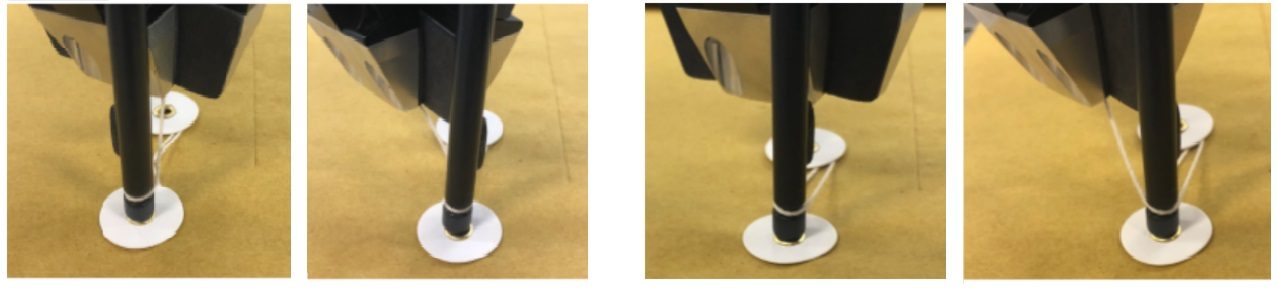
\includegraphics[height=35mm]{chapters/figures/experiments/exp2_CWCCW2.jpg}
	\caption{CW case on the left and CCW case on the right for r = 3 mm.}
	\label{fig:CWCCW2}
\end{figure}

Let's see the results for torques in Table~\ref{tab:3mm}.
% Table generated by Excel2LaTeX from sheet 'CW P1'
\begin{table}[htbp]
	\centering
	\begin{tabular}{|l|c|c|c|}
		\cmidrule{2-4}    \multicolumn{1}{r|}{} & \multicolumn{3}{c|}{\textbf{r = 3 mm}} \\
		\cmidrule{2-4}    \multicolumn{1}{r|}{} & \textbf{$|M_{x, tension} - M_{x, no tension}|$} & \textbf{$|M_{y, tension} - M_{y, no tension}|$} & Comparison to threshold \\
		\cmidrule{1-4}
		\textbf{CW case} & $0.254 N \cdot m$ & $0.185 N \cdot m$ & $> 0.095 N \cdot m$ \\
		\midrule
		\textbf{CCW case} & $0.020 N \cdot m$ & $0.056 N \cdot m$ & $< 0.095 N \cdot m$ \\
		\bottomrule
	\end{tabular}%
	\caption{Results for torque values in CW and CCW case for r = 3mm.}
	\label{tab:3mm}%
\end{table}%

We appreciate the same as in the previous case. In CW case both $|\Delta M_{x}|$ and $| \Delta M_{y}|$ are greater than threshold value while in CCW case they are smaller. We can thus distinguish both cases for a pivot's radius of 3 mm.

Let's see now what happens with a radius of 2 mm.

\subsection{Radius = 2 mm}
For this experiment, we took an Allen key with a 2 mm radius and we winded the string around it CW and then CCW. Both cases are shown in Figure~\ref{fig:CWCCW3}:
\begin{figure}[h!]
	\centering
	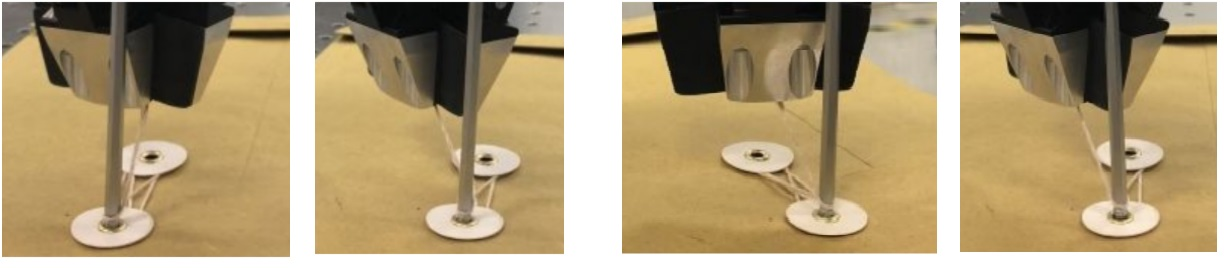
\includegraphics[height=35mm]{chapters/figures/experiments/exp2_CWCCW3.jpg}
	\caption{CW case on the left and CCW case on the right case for r = 2 mm.}
	\label{fig:CWCCW3}
\end{figure}

The results for torques are shown in Table~\ref{tab:2mm}.
% Table generated by Excel2LaTeX from sheet 'CW P1'
\begin{table}[htbp]
	\centering
	\begin{tabular}{|l|c|c|c|}
		\cmidrule{2-4}    \multicolumn{1}{r|}{} & \multicolumn{3}{c|}{\textbf{r = 2 mm}} \\
		\cmidrule{2-4}    \multicolumn{1}{r|}{} & \textbf{$|M_{x, tension} - M_{x, no tension}|$} & \textbf{$|M_{y, tension} - M_{y, no tension}|$} & Comparison to threshold \\
		\cmidrule{1-4}
		\textbf{CW case} & $0.405 N \cdot m$ & $0.320 N \cdot m$ & $> 0.095 N \cdot m$ \\
		\midrule
		\textbf{CCW case} & $0.566 N \cdot m$ & $0.407 N \cdot m$ & $> 0.095 N \cdot m$ \\
		\bottomrule
	\end{tabular}%
	\caption{Results for torque values in CW and CCW case for r = 2mm.}
	\label{tab:2mm}%
\end{table}%

In this case, we see that both in CW and CCW case, if the gripper moves $2 \cdot r_{p}$ in perpendicular to pivots' joining axis,  $|\Delta M_{x}|$ and $| \Delta M_{y}|$ are greater than threshold value. In this case we can thus not distinguish between CW and CCW case. For this algorithm to work with this force/torque sensor, pivots' radius must be bigger than 2 mm. A radius of 2 mm or smaller could be considered as negligible.

\section{Experiment 3: Minimum distance between pivots}
In this section we show different experiments where we modify the distance between pivots to figure out which is the minimum distance we could have for the force/torque sensor to distinguish between P1 and P2.

Let's start by analyzing what happens with the real distance between pivots (4.25 cm).

\subsection{Distance = 4.25 cm}
For this experiment, we first tied the string around P1 and then about P2 and we took torque values when the gripper moved $2 \cdot r_{p}$ in perpendicular to pivots' joining axis.

In Figure~\ref{fig:distance1} this first experiment is shown:
\begin{figure}[h!]
	\centering
	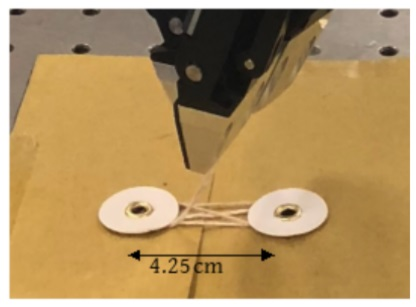
\includegraphics[height=40mm]{chapters/figures/experiments/exp3_distance1.jpg}
	\caption{First experiment with a distance of 4.25 cm between pivots.}
	\label{fig:distance1}
\end{figure}

Values for torques when the string is tied about P1 and when the string is tied about P2 are shown in Table~\ref{tab:distance1} below.
% Table generated by Excel2LaTeX from sheet 'CW P1'
\begin{table}[htbp]
	\centering
	\begin{tabular}{|l|c|c|c|c|}
		\cmidrule{2-5}    \multicolumn{1}{r|}{} & \multicolumn{4}{c|}{\textbf{d = 4.25 cm}} \\
		\cmidrule{2-5}    \multicolumn{1}{r|}{} & \multicolumn{1}{l|}{\textbf{$M_{x, no tension}$}} & \textbf{$M_{x, tension}$} & \textbf{$M_{x, tension} - M_{x, no tension}$} & Comparison to threshold \\
		\midrule
		\textbf{P1} & $0.026 N \cdot m$ & $-0.134 N \cdot m$ & $-0.160 N \cdot m$ & $< -0.095 N \cdot m$ \\
		\midrule
		\textbf{P2} & $-0.035 N \cdot m$ & $0.067 N \cdot m$ & $0.102 N \cdot m$ & $> 0.095 N \cdot m$ \\
		\bottomrule
	\end{tabular}%
	\caption{Results for torque values when the string is tied about P1 and about P2 for a distance of 4.25 cm between pivots.}
	\label{tab:distance1}%
\end{table}%

In the case where the string is tied about P1, $\Delta M_{x}$ is less than the negative value of the threshold when the gripper moves $2 \cdot r_{p}$, while when the string is tied about P2, $\Delta M_{x}$ is greater than the positive value of the threshold. We can thus distinguish if the string is tied about P1 or P2 for a distance of 4.25 cm between pivots (real case).

Let's see what happens for a distance of 3.5 cm between pivots.

\subsection{Distance = 3.5 cm}
For this experiment, we did the same thing as in the previous one but we changed pivots' distance to 3.5 cm. This is shown in Figure~\ref{fig:distance2} below:
\begin{figure}[h!]
	\centering
	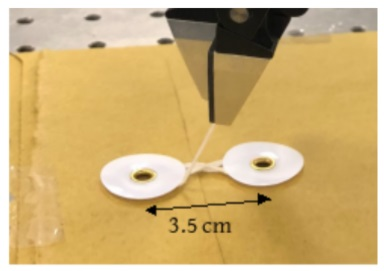
\includegraphics[height=40mm]{chapters/figures/experiments/exp3_distance2.jpg}
	\caption{Experiment with a distance of 3.5 cm between pivots.}
	\label{fig:distance2}
\end{figure}

Values for torques when the string is tied about P1 and when the string is tied about P2 are shown in Table~\ref{tab:distance2} below.
% Table generated by Excel2LaTeX from sheet 'CW P1'
\begin{table}[htbp]
	\centering
	\begin{tabular}{|l|c|c|c|c|}
		\cmidrule{2-5}    \multicolumn{1}{r|}{} & \multicolumn{4}{c|}{\textbf{d = 3.5 cm}} \\
		\cmidrule{2-5}    \multicolumn{1}{r|}{} & \multicolumn{1}{l|}{\textbf{$M_{x, no tension}$}} & \textbf{$M_{x, tension}$} & \textbf{$M_{x, tension} - M_{x, no tension}$} & Comparison to threshold \\
		\midrule
		\textbf{P1} & $0.004 N \cdot m$ & $-0.097 N \cdot m$ & $-0.101 N \cdot m$ & $< -0.095 N \cdot m$ \\
		\midrule
		\textbf{P2} & $-0.032 N \cdot m$ & $0.073 N \cdot m$ & $0.105 N \cdot m$ & $> 0.095 N \cdot m$ \\
		\bottomrule
	\end{tabular}%
	\caption{Results for torque values when the string is tied about P1 and about P2 for a distance of 3.5 cm between pivots.}
	\label{tab:distance2}%
\end{table}%

Again, in this case as in the previous one, when the string is tied about P1, $\Delta M_{x}$ is less than the negative value of the threshold, while when the string is tied about P2, $\Delta M_{x}$ is greater than the positive value of the threshold. We can thus distinguish whether the string is tied about P1 or P2 for a distance of 3.5 cm between pivots.

Let's see now what happens for a distance of 3 cm between pivots.

\subsection{Distance = 3 cm}
For this experiment, we changed pivots' distance to 3 cm. This is shown in Figure~\ref{fig:distance3} below:
\begin{figure}[h!]
	\centering
	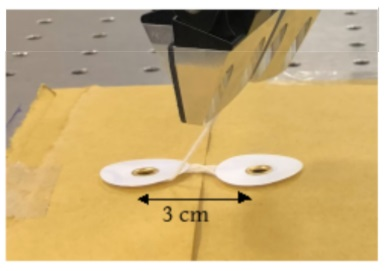
\includegraphics[height=40mm]{chapters/figures/experiments/exp3_distance3.jpg}
	\caption{Experiment with a distance of 3 cm between pivots.}
	\label{fig:distance3}
\end{figure}

Values for torques when the string is tied about P1 and when the string is tied about P2 are shown in Table~\ref{tab:distance3} below.
% Table generated by Excel2LaTeX from sheet 'CW P1'
\begin{table}[htbp]
	\centering
	\begin{tabular}{|l|c|c|c|c|}
		\cmidrule{2-5}    \multicolumn{1}{r|}{} & \multicolumn{4}{c|}{\textbf{d = 3 cm}} \\
		\cmidrule{2-5}    \multicolumn{1}{r|}{} & \multicolumn{1}{l|}{\textbf{$M_{x, no tension}$}} & \textbf{$M_{x, tension}$} & \textbf{$M_{x, tension} - M_{x, no tension}$} & Comparison to threshold \\
		\midrule
		\textbf{P1} & $0.033 N \cdot m$ & $-0.026 N \cdot m$ & $-0.007 N \cdot m$ & $> -0.095 N \cdot m$ \\
		\midrule
		\textbf{P2} & $0.032 N \cdot m$ & $0.046 N \cdot m$ & $0.014 N \cdot m$ & $< 0.095 N \cdot m$ \\
		\bottomrule
	\end{tabular}%
	\caption{Results for torque values when the string is tied about P1 and about P2 for a distance of 3 cm between pivots.}
	\label{tab:distance3}%
\end{table}%

In this case, when the string is tied about P1 as well as when it is tied about P2, $|\Delta M_{x}|$ is less than the the threshold value, when the gripper moves $2 \cdot r_{p}$. We can thus not know which pivot the string is tied about for a distance of 3 cm between pivots or less.

\section{Experiment 4: Comparison of robot fail ratio with human fail ratio}
For this experiment we performed 30 tests where the robot had to open the envelope that had been previously tied arbitrarily. Then, we performed this same 30 tests with 5 different human being with closed eyes, so they were in the same conditions than the robot. Finally we compared the results to see who succeed more times.

Let's start by seeing robot results of success and fails in Table~\ref{tab:exp4_robot}.
% Table generated by Excel2LaTeX from sheet 'CW P1'
\begin{table}[htbp]
	\centering
	\begin{tabular}{|l|c|}
		\cmidrule{2-2}    \multicolumn{1}{r|}{} & \textbf{Robot} \\
		\midrule
		\textbf{Success} & 19 \\
		\midrule
		\textbf{Fails} & 11 \\
		\bottomrule
	\end{tabular}%
	\caption{Number of success and fails made by the robot in the 30 experiments.}
	\label{tab:exp4_robot}%
\end{table}%

The robot succeded 19 times to open the envelope and failed 11 out of 30 attempts. The reasons why the robot failed are:
\begin{itemize}
 \item Bad reading of the torque by the sensor: a bad reading of torque makes the robot to take the wrong action. For example, it turns around the wrong pivot or in the wrong direction.
 \item Error in the movement of the robot: if there is an error in the movement and the spiral movement is not perfect, the gripper may pull the string too much during the movement (and break it) or it may not finish the turn where it is supposed to and the envelope will not be opened.
\end{itemize}

Let's see now the results for humans. In Figure~\ref{fig:humans} we can see how the experiment was performed by the 5 people:
\begin{figure}[h!]
	\centering
	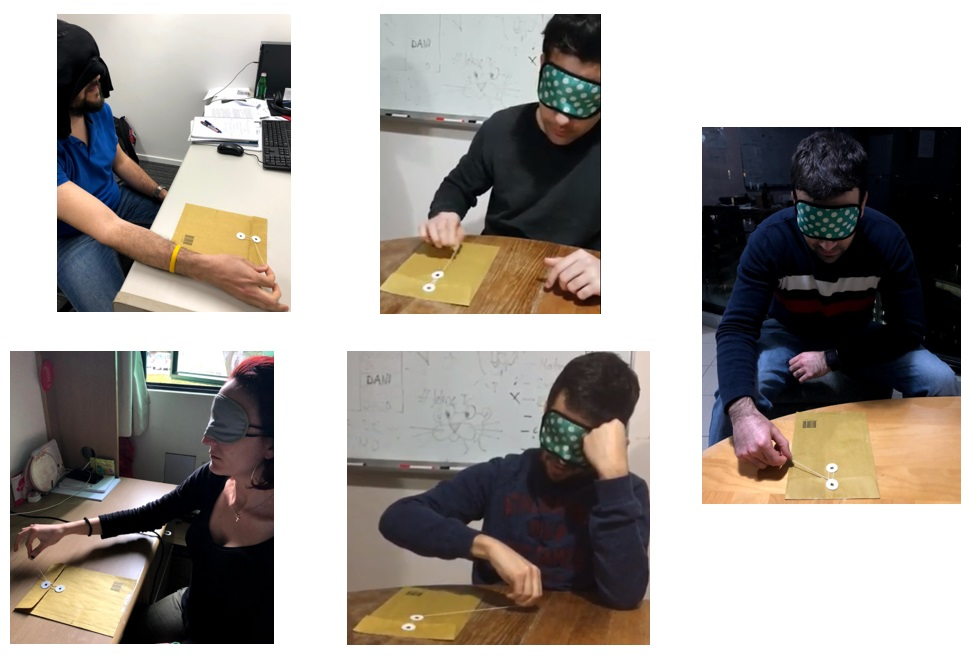
\includegraphics[height=80mm]{chapters/figures/experiments/exp4_humans.jpg}
	\caption{Experiment performed by 5 people with closed eyes trying to open the envelope.}
	\label{fig:humans}
\end{figure}

In Table~\ref{tab:humans}, the results for these 5 people are shown:\newline
% Table generated by Excel2LaTeX from sheet 'CW P1'
\begin{table}[h!]
	\centering
	\begin{tabular}{|l|c|c|c|c|c|}
		\cmidrule{2-6}    \multicolumn{1}{r|}{} & \textbf{Human 1} & \textbf{Human 2} & \textbf{Human 3} & \textbf{Human 4} & \textbf{Human 5} \\
		\midrule
		\textbf{Success} & 12    & 21    & 17    & 7     & 26 \\
		\midrule
		\textbf{Fails} & 18    & 9     & 13    & 23    & 4 \\
		\bottomrule
	\end{tabular}%
	\caption{Number of success and fails made by the 5 people in the 30 experiments.}
	\label{tab:humans}%
\end{table}%

We appreciate that results for different humans are very different. That is why we took different people to perform the experiments, because every person is different while the algorithm for the robot will always work the same way.
The reasons why people failed are:
\begin{itemize}
	\item They did not know which direction to turn.
	\item They did not know where they were in the space and they gave up.
	\item They thought the envelope was already opened and it was not.
\end{itemize}

Let's compare now the percentage of success for the robot and for an average person in Table~\ref{tab:comprobothuman}:
% Table generated by Excel2LaTeX from sheet 'CW P1'
\begin{table}[htbp]
	\centering
	\begin{tabular}{|l|c|c|}
		\cmidrule{2-3}    \multicolumn{1}{r|}{} & \textbf{Robot} & \textbf{Humans} \\
		\midrule
		\textbf{Percentage of success} & 63.30\% & 55.30\% \\
		\bottomrule
	\end{tabular}%
	\caption{Comparison between robot percentage of success and human percentage of success.}
	\label{tab:comprobothuman}%
\end{table}%

We see that the percentage of success for the robot is higher than for an average human. 

The main difference between humans and the robot was that people could correct their movement if they realized they were doing it wrong, while the robot is not able to correct the movement and will not open the envelope if it doesn't figure out the good movement the first time.

We also noticed that when a person succeded to open the envelope, he or she took much less time than the robot. The robot takes around 4 minutes to open the envelope while the human did it in about 30 seconds.


\chapter{CONCLUSION AND FUTURE LINES}
\label{ch:Conclusion and Future Lines}

\section{Conclusion}
To conclude this work we can say that the algorithm to open the envelope works correctly. The spiral movement is a good approach to plan the trajectory of the end enfector in order to unwound the string form the circular pivots. We have demonstrated that it is possible for a robot to open a string-envelope only with a wrist force/torque sensor. Furthermore, even if the algorithm is not perfect, it succeeds more than an average human in the same conditions.

\section{Future Lines}
In order to continue developing this project, we could add corrective movements. We saw that when humans succeeded to open the envelope, it was because they were able to correct their movement. If we add corrective movements to the robot, its percentage of success could increase.

We also noticed that when humans opened the envelope correctly, they did it in less time than the robot. The speed of the robot's movement can be increased to such point that it could be much faster than a human. We could add superhuman capabilities to the robot by increasing its speed, so it would open the envelope in less than 5 seconds.

In order to enhance autonomy, other sensors such as visual sensing could be added to the robot. If we provide the robot with visual sensing, it could for example detect the end of the string at the beginning and grasp it, or measure the distance between pivots and pivots' radius. This way, we would get rid of the preconditions we have and the algorithm would become more general and work in many different situations and with different parameters of envelopes.

Finally, we created a project on GitHub (Figure~\ref{fig:github}). This is a platform for collaborative development that contains from open source projects to private team repositories. There, developers can discover, share, and build better software. The repository created for this project is called "envelope" and it can be found in the following link: https://github.com/irunegoizueta/envelope/. There, we can find all the executables needed for the algorithm to work correctly and an explanation of how to install and run them.
\begin{figure}[htbp]
	\centering
	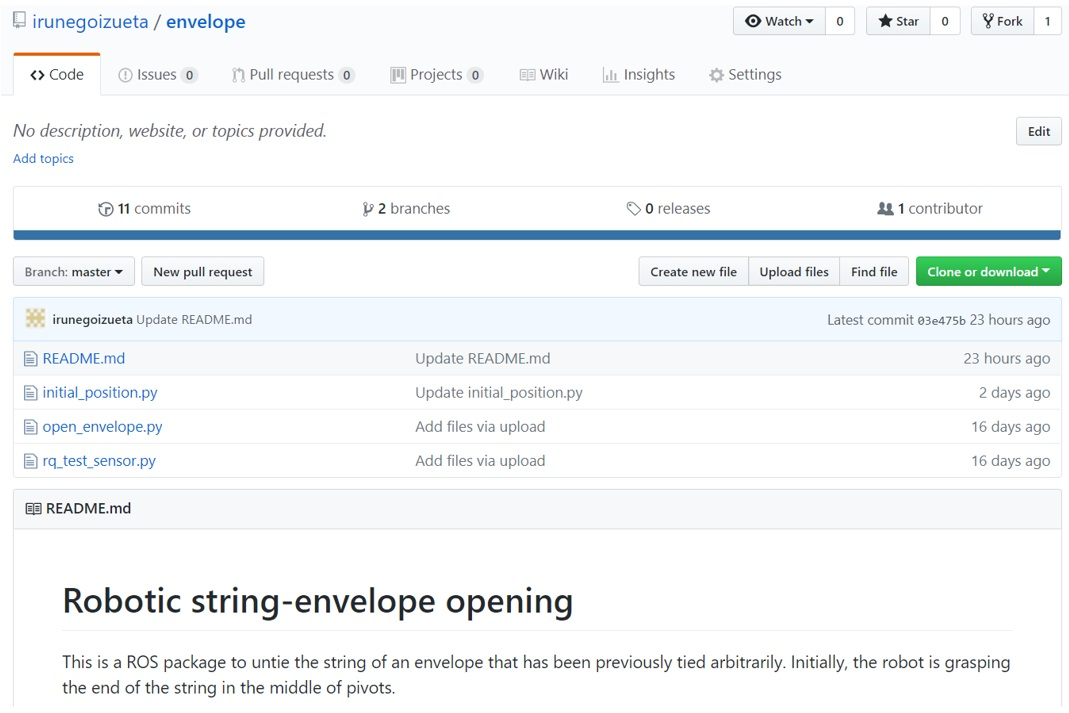
\includegraphics[height=110mm]{chapters/figures/conclusion/github.jpg}
	\caption{Repository "envelope" on GitHub.}
	\label{fig:github}
\end{figure}


\chapter{BUDGET}
\label{ch:budget}
Here, we show the budget corresponding to the development of this project. This one is split in different lines:
\begin{itemize}
	\item \underline{Consumables}: The consumables used in this project are the string-envelopes.
	\item \underline{Equipment}: The equipment used in this work is the UR10 robot, the Robotiq force/torque sensor, the Robotiq 3 finger gripper and the computer.
	\item \underline{Software}: Here we find Ubuntu 16.04.3 LTS, Windows 10 and ROS.
	\item \underline{Labour}: This line corresponds to the engineering hours spent on this work.
\end{itemize}

In Table~\ref{tab:consumables} below, the budget for consumables is shown:
% Table generated by Excel2LaTeX from sheet 'Hoja1'
\begin{table}[h!]
	\centering
	\begin{tabular}{p{8em}cccc}
		\toprule
		{Quantity} & \multicolumn{1}{c}{{Reference}} & \multicolumn{1}{c}{{Description}} &  \multicolumn{1}{p{8em}}{Unitary Price (\$)} & \multicolumn{1}{p{8em}}{Total Price (\$)} \\
		\midrule
		\multicolumn{1}{p{4em}}{20} & 65035 & \multicolumn{1}{p{8em}}{String-Envelope} & 1.4   & 28 \\
		\midrule
		\multicolumn{1}{p{12em}}{Total consumables} &       &       &       & 28 \\
		\bottomrule
	\end{tabular}%
	\caption{Budget for consumables.}
	\label{tab:consumables}%
\end{table}%

Table~\ref{tab:equipment} shows the budget for the equipment used in this project:
% Table generated by Excel2LaTeX from sheet 'Hoja1'
\setlength\LTpost{0pt}
\begin{longtable} {p{6em}cccccc}
		\toprule
		Equipment & \multicolumn{1}{p{6.5em}}{Cost of acquisition (\$)} & \multicolumn{1}{p{7em}}{Depreciation period (years)} & \multicolumn{1}{p{9em}}{Depreciation mensual cost (\$)} & \multicolumn{1}{p{6em}}{Time of use (month)} & \multicolumn{1}{p{3em}}{Depreciation (\$)} \\
		\midrule
		Robot & 50000 & 4     & 1041  & 6     & 6246 \\
		\midrule
		Force/Torque Sensor & 4000  & 4     & 83    & 6     & 498 \\
		\midrule
		Gripper & 18000 & 4     & 375   & 6     & 2250 \\
		\midrule
		Computer & 700   & 4     & 15    & 6     & 90 \\
		\midrule
		Total equipment &       &       &       &       & 9084 \\
		\bottomrule
	\caption{Budget for equipment.}
	\label{tab:equipment}%
\end{longtable}%

The budget for the software is shown in Table~\ref{tab:software}:
% Table generated by Excel2LaTeX from sheet 'Hoja1'
\begin{table}[h!]
	\centering
	\begin{tabular}{p{6em}ccccc}
		\toprule
		Software & \multicolumn{1}{p{6.5em}}{Cost of acquisition (\$)} & \multicolumn{1}{p{7em}}{Depreciation period (years)} & \multicolumn{1}{p{9em}}{Depreciation mensual cost (\$)} & \multicolumn{1}{p{6em}}{Time of use (month)} & \multicolumn{1}{p{3em}}{Depreciation (\$)} \\
		\midrule
		Ubuntu 16.04.3 LTS & 0     & \multicolumn{1}{p{7em}}{-} & \multicolumn{1}{p{9em}}{-} & 6     & \multicolumn{1}{p{3em}}{-} \\
		\midrule
		Windows 10 & 12000 & 1     & 1000  & 1     & 1000 \\
		\midrule
		ROS   & 0     & \multicolumn{1}{p{7em}}{-} & \multicolumn{1}{p{9em}}{-} & 6     & \multicolumn{1}{p{3em}}{-} \\
		\midrule
		Total software &       &       &       &       & 1000 \\
		\bottomrule
	\end{tabular}%
	\caption{Budget for the software.}
	\label{tab:software}%
\end{table}%

Finally, the budget for the labour is shown in Table~\ref{tab:labour}:
% Table generated by Excel2LaTeX from sheet 'Hoja1'
\begin{table}[h!]
	\centering
	\begin{tabular}{p{6.18em}ccc}
		\toprule
		{Task} & \multicolumn{1}{c}{{Duration (hours)}} &  \multicolumn{1}{p{8em}}{Unitary Price (\$)} & \multicolumn{1}{p{8em}}{Total Price (\$)} \\
		\midrule
		Engineering & 960   & 50    & 48000 \\
		\midrule
		Total labour &       &       & 48000 \\
		\bottomrule
	\end{tabular}%
	\caption{Budget for the labour.}
	\label{tab:labour}%
\end{table}%

The summary of the global budget for this project amounts to 77347 \$ and is presented in Table~\ref{tab:global}:
% Table generated by Excel2LaTeX from sheet 'Hoja1'
\begin{table}[h!]
	\centering
	\begin{tabular}{ccc}
		\toprule
		Line  & \multicolumn{1}{p{5.5em}}{Partial Amount (\$)} & \multicolumn{1}{p{5.5em}}{Accumulated Amount (\$)} \\
		\midrule
		Consumables & 28    & 28 \\
		\midrule
		Equipment & 9084  & 9112 \\
		\midrule
		Software & 1000  & 10112 \\
		\midrule
		Labour & 48000 & 58112 \\
		\midrule
		Indirect costs (10\%) &       & 5811.2 \\
		\midrule
		Total without VAT &       & 63923.2 \\
		\midrule
		Total with VAT &       & 77347 \\
		\bottomrule
	\end{tabular}%
\caption{Summary of the global budget for this project.}
\label{tab:global}%
\end{table}%



%Configuración particular de las cabeceras y pies de página de los ejercicios

%\renewcommand{\thechapter}{\roman{chapter}}
%\def\chaptername{Exercises}
%\setcounter{chapter}{0}
%\renewcommand{\chaptermark}[1]{\markboth{Exercises \thechapter. #1}{}} %configuración de las cabeceras
%\renewcommand{\sectionmark}[1]{\markright{Exercises \thechapter. #1}}
%
%% programaci'on de robots industriales
%\include{1_robot_intro/CPR_introduction}
%
%\part{Laboratory exercises}
%%pr�cticas
%%\graphicspath{{./practicas/matlab/figures/}}
%
%\graphicspath{{./}}
%
%
%%%%%%%%%%%%%%%%%% Exams
%\part{Exams}
%
%%Configuración particular de las cabeceras y pies de página de los examenes
%
%\renewcommand{\thechapter}{\alph{chapter}}
%\def\chaptername{Exams}
%\setcounter{chapter}{0}
%\renewcommand{\chaptermark}[1]{\markboth{Exams \thechapter. #1}{}} %configuración de las cabeceras
%\renewcommand{\sectionmark}[1]{\markright{Exams \thechapter. #1}}
%
%%ex'amenes de rob'otica industrial
%% programaci'on de robots industriales
%\include{1_robot_intro/CPR_introduction}
%
%%%%%%%%%%%%%%%%% Appendix
%\part{Appendix}
%\begin {appendix}
%%Configuración particular de las cabeceras y pies de página del appendix
%\renewcommand{\chaptermark}[1]{\markboth{Appendix \thechapter. #1}{}} %configuración de las cabeceras
%\renewcommand{\sectionmark}[1]{\markright{Appendix Section \thesection. #1}}
%
%% programaci'on de robots industriales
%\include{1_robot_intro/CPR_introduction}
%
%\end{appendix}

\backmatter

%%%%%%%%%%%%%%%% Final del libro
%índice de materias
\printindex


%es el turno de la bibliografía
\bibliographystyle{plain}
\nocite{*} % imprime toda la bibliografía, aunque no esté citada
\bibliography{Bibliography}

\end{document}



